%%%%%%%%%%%%%%%%%%%%%%%%%%%%%%%%%%%%%%%%%%%%%%%%%%%%%%%%%
%%   $RCSfile: hpsg04.tex,v $
%%  $Revision: 1.1 $
%%      $Date: 2004/08/11 09:53:01 $
%%     Author: Stefan Mueller (CL Uni Bremen)
%%    Purpose: 
%%   Language: LaTeX
%%%%%%%%%%%%%%%%%%%%%%%%%%%%%%%%%%%%%%%%%%%%%%%%%%%%%%%%%
%%
%% $Log: hpsg04.tex,v $
%% Revision 1.1  2004/08/11 09:53:01  stefan
%% *** empty log message ***
%%
%% Revision 1.1  2003/10/12 13:42:57  stefan
%% Initial revision
%%
%%%%%%%%%%%%%%%%%%%%%%%%%%%%%%%%%%%%%%%%%%%%%%%%%%%%%%%%%

\documentclass[11pt,a4paper,fleqn]{article}
\usepackage{times}
\thispagestyle{empty}



\usepackage[T1]{fontenc}   % Silbentrennung

\usepackage{8bit}

\usepackage[bookmarks=true,bookmarksopen=true,%
breaklinks=true,%
draft=false,colorlinks=false,plainpages=false,hyperfootnotes=false,%
linkcolor=black,%
pagecolor=black,%
pdfauthor={Stefan M�ller (Editor)},%
pdftitle={Proceedings of the HPSG06 Conference},%
pdfkeywords={HPSG}%,
pdftex=true%
%ps2pdf=true  %ohne diesen Treiber geht der Zeilenumbruch in URLs
]{hyperref}% for pdf files

\usepackage{pdfpages}


\hypersetup{colorlinks=false, pdfborder={0 0 0}}

\begin{document}

\begin{center}
{\Large
                 Proceedings of the HPSG06 Conference\\[\baselineskip]

Linguistic Modelling Laboratory\\
Institute for Parallel Processing\\
Bulgarian Academy of Sciences\\
Sofia\\
Held In Varna\\[\baselineskip]

                        Stefan M{\"u}ller (Editor)\\[\baselineskip]

                                2006\\[\baselineskip]

                          CSLI Publications\\[\baselineskip]

              http://csli-publications.stanford.edu/
}
\end{center}
\newpage
\tableofcontents

\newpage

\section{Editor's Note}

The 13th International Conference on Head-Driven Phrase Structure Grammar (2006) was held in Varna
and organized by the Linguistic Modelling Laboratory of the Institute for Parallel Processing of the
Bulgarian Academy of Sciences in Sofia.

The conference featured 2 invited talks, 16 papers, and 4 posters
selected by the program committee 
(Anne Abeill�,
Raul Aranovich,
Emily Bender,
Gosse Bouma,
Ant�nio Branco,
Chan Chung,
Ann Copestake,
Berthold Crysmann,
Elisabeth Engdahl,
Anna Feldman,
Dan Flickinger,
Howard Gregory,
Daniele Godard,
Erhard Hinrichs (chair),
Jong-Bok Kim,
Valia Kordoni,
Ania Kupsc,
Shalom Lappin,
Robert Levine,
Stefan M�ller,
Tsuneko Nakazawa,
Petya Osenova,
Gerald Penn,
Luisa Sadler,
Ivan Sag,
Manfred Sailer,
Gautam Sengupta,
Jan-Philipp Soehn (chair),
Jesse Tseng,
Nathan Vaillette,
Stephen Wechsler,
Eun-Jung Yoo,
Larisa Zlatic).

A workshop about \emph{Regularity and Irregularity in Grammar and Language}
was attached to the conference. It featured one invited talk
and 5 papers, selected by the program committee.

In total there were 39 submissions to the main conference and  submissions to the
workshop. %<!--, which gives an acceptance rate of %.-->
We want to thank the respective program committee for putting this nice program together.




Thanks go to Kiril Simov and Petya Osenova, who were in charge of local arrangements.


As in the past years the contributions to the conference proceedings are based on the five page abstract
that was reviewed by the respective program committees, but there is no additional reviewing of the
longer contribution to the proceedings.
To ensure easy access and fast publication we have chosen an electronic format.


The proceedings include all the papers except those by Stefan M�ller, Shravan Vasishth, and Frank
van Eynde.



\newpage
\part{Contributions to the Main Conference}




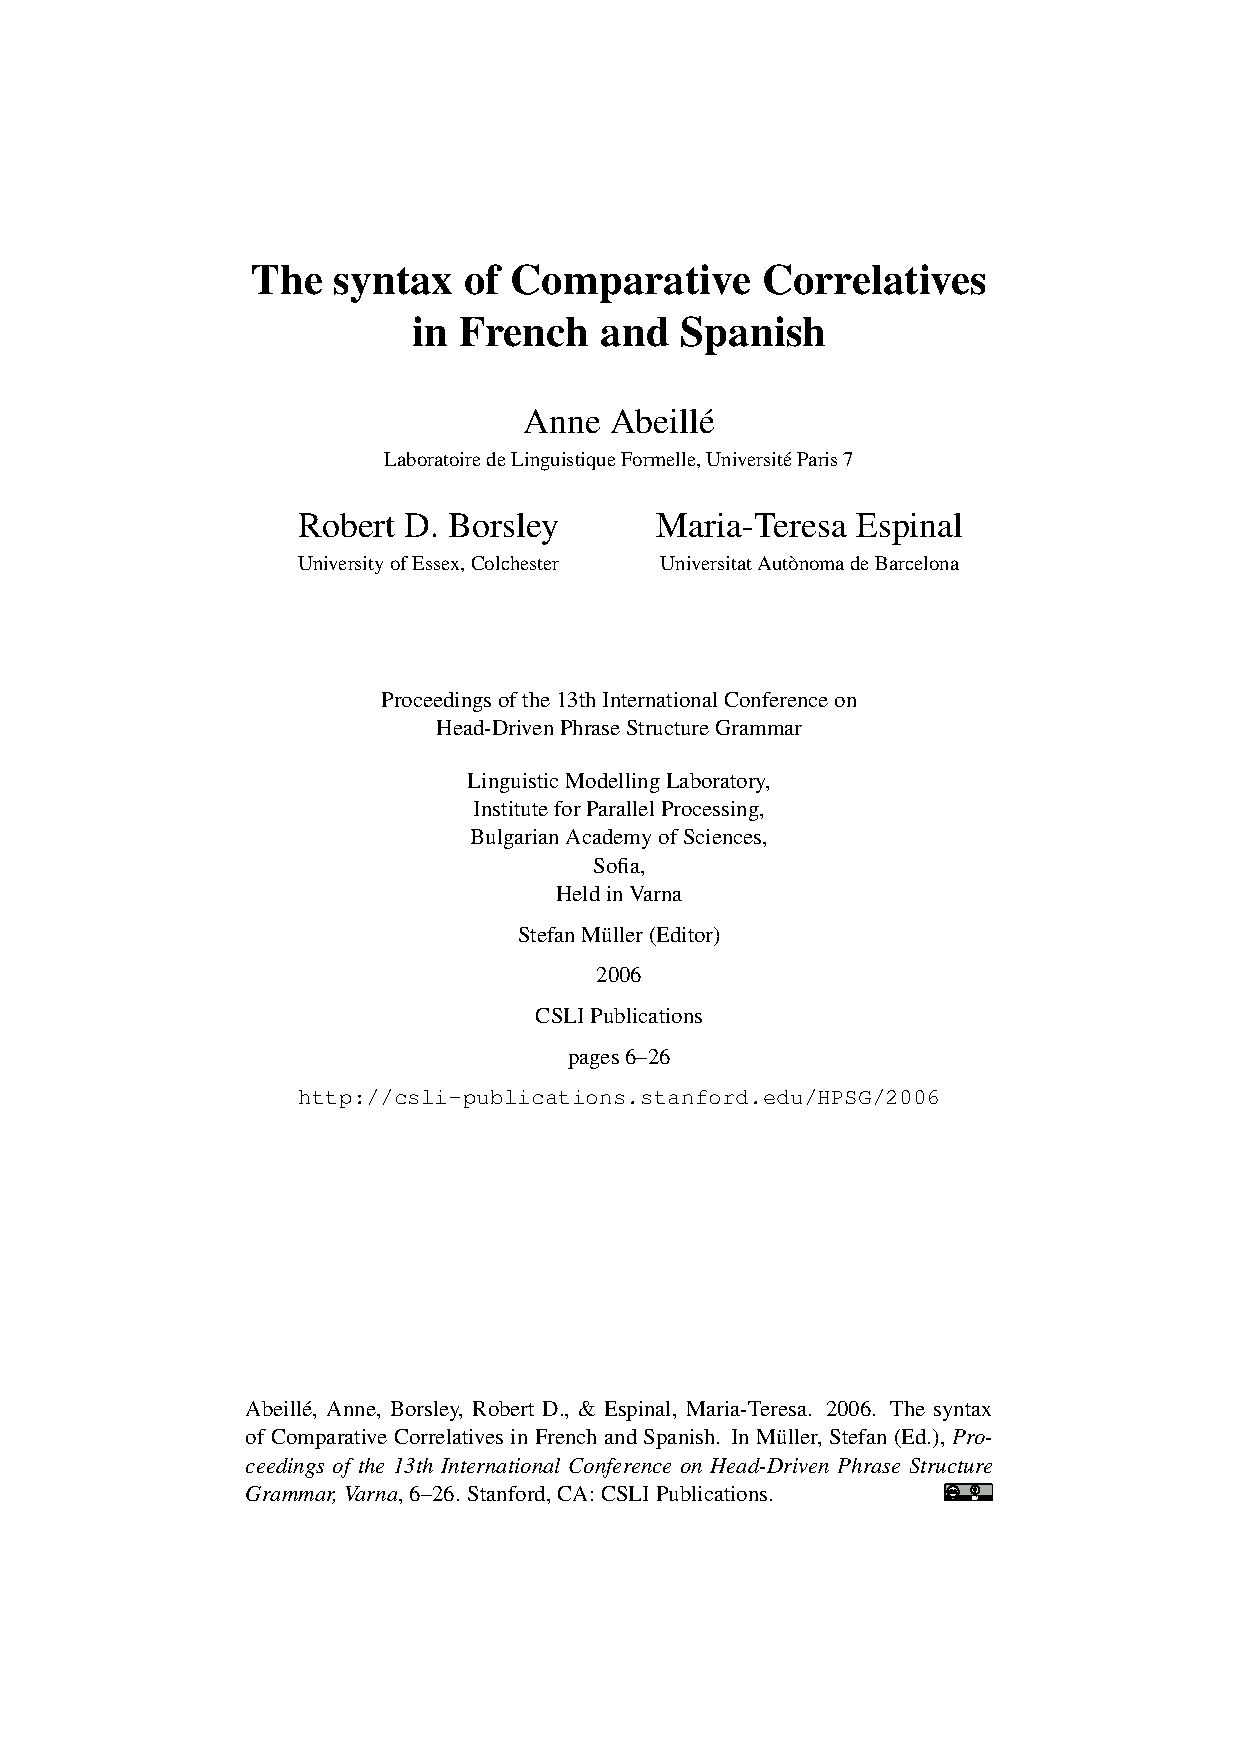
\includepdf[pages=-,pagecommand=\thispagestyle{plain},
            addtotoc={1,section,1,
            {Anne Abeill�, Robert D. Borsley, and Maria-Teresa Espinal: The syntax of Comparative Correlatives in French and Spanish},
             abe}]{abe.pdf}

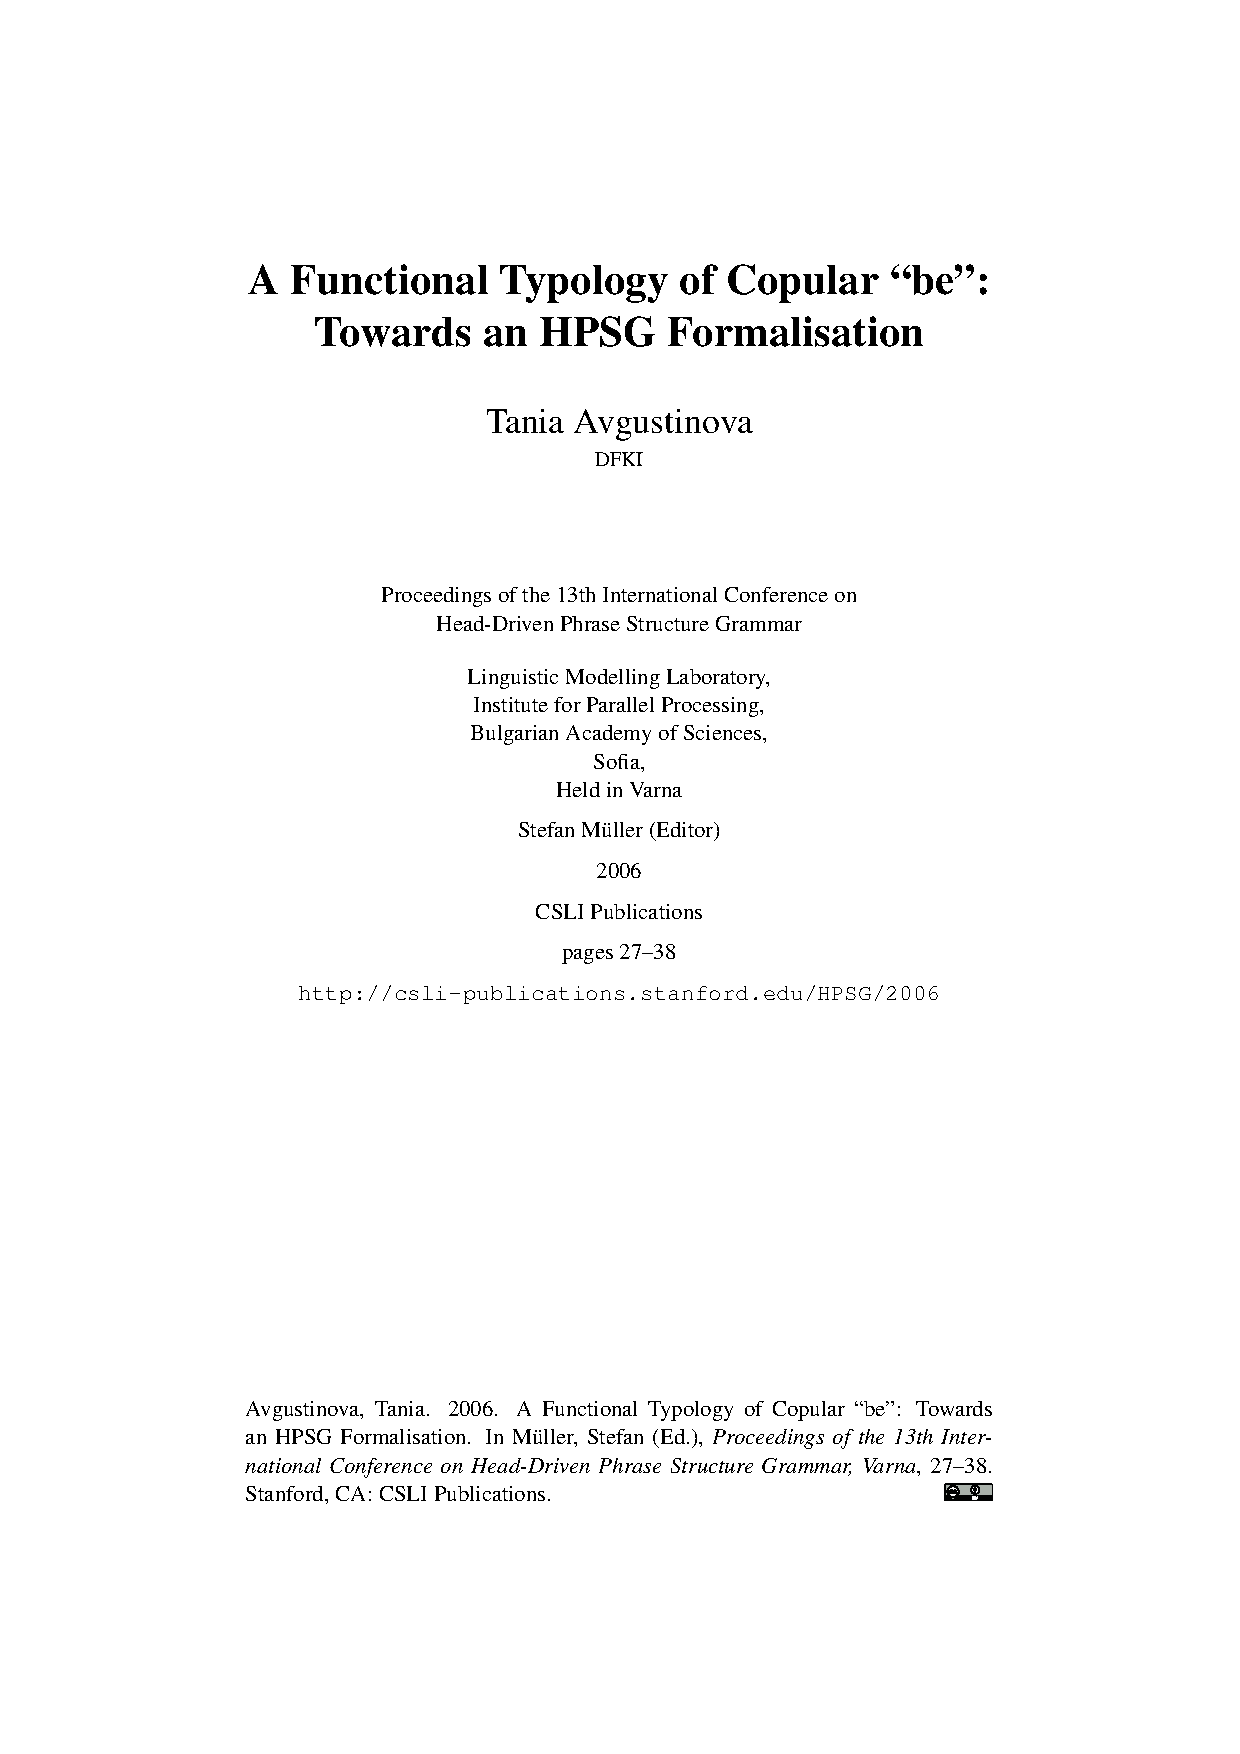
\includepdf[pages=-,pagecommand=\thispagestyle{plain},
            addtotoc={1,section,1,
            {Tania Avgustinova: A Functional Typology of Copular ``be'': Towards an HPSG Formalisation},
             avgustinova}]{avgustinova.pdf}

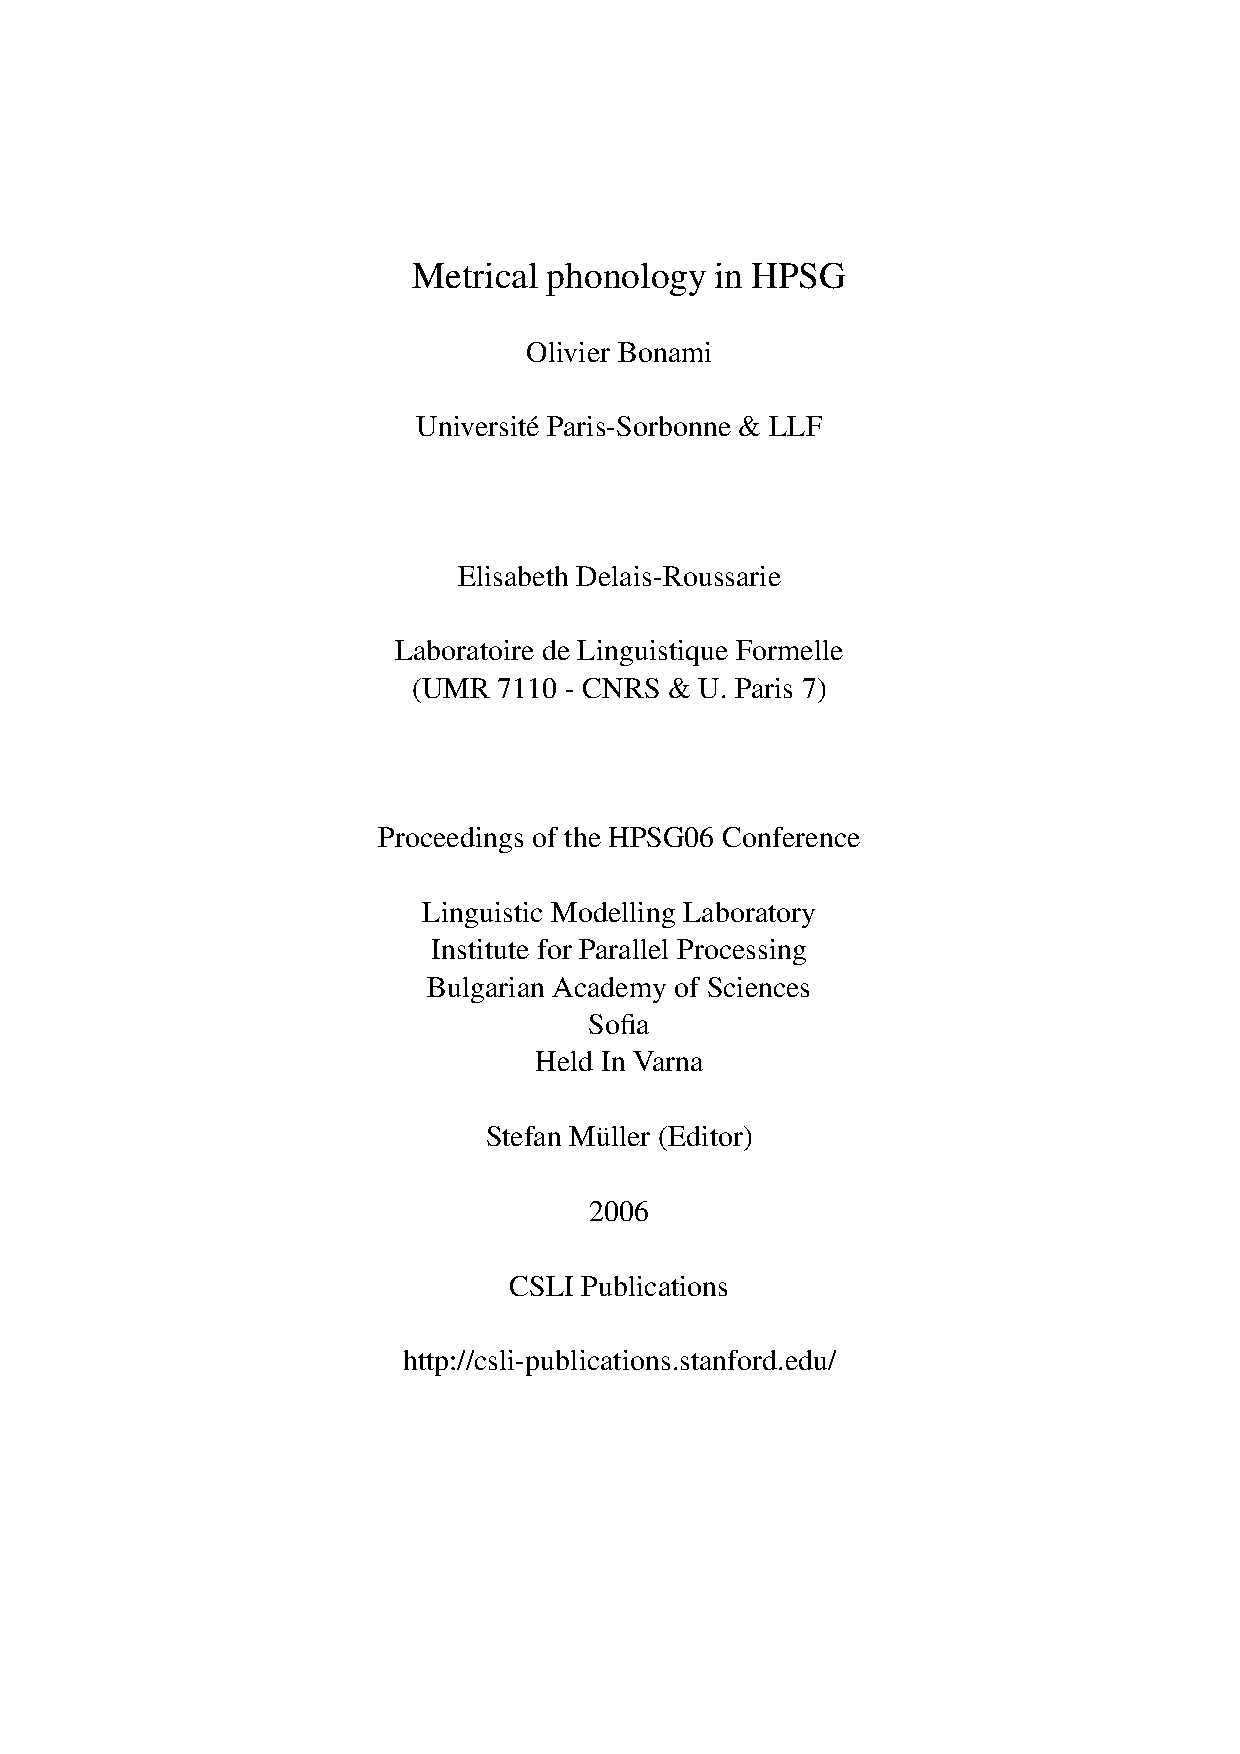
\includepdf[pages=-,pagecommand=\thispagestyle{plain},
            addtotoc={1,section,1,
            {Olivier Bonami and Elisabeth Delais-Roussarie: Metrical Phonology in HPSG},
             bonami-delais}]{bonami-delais.pdf}

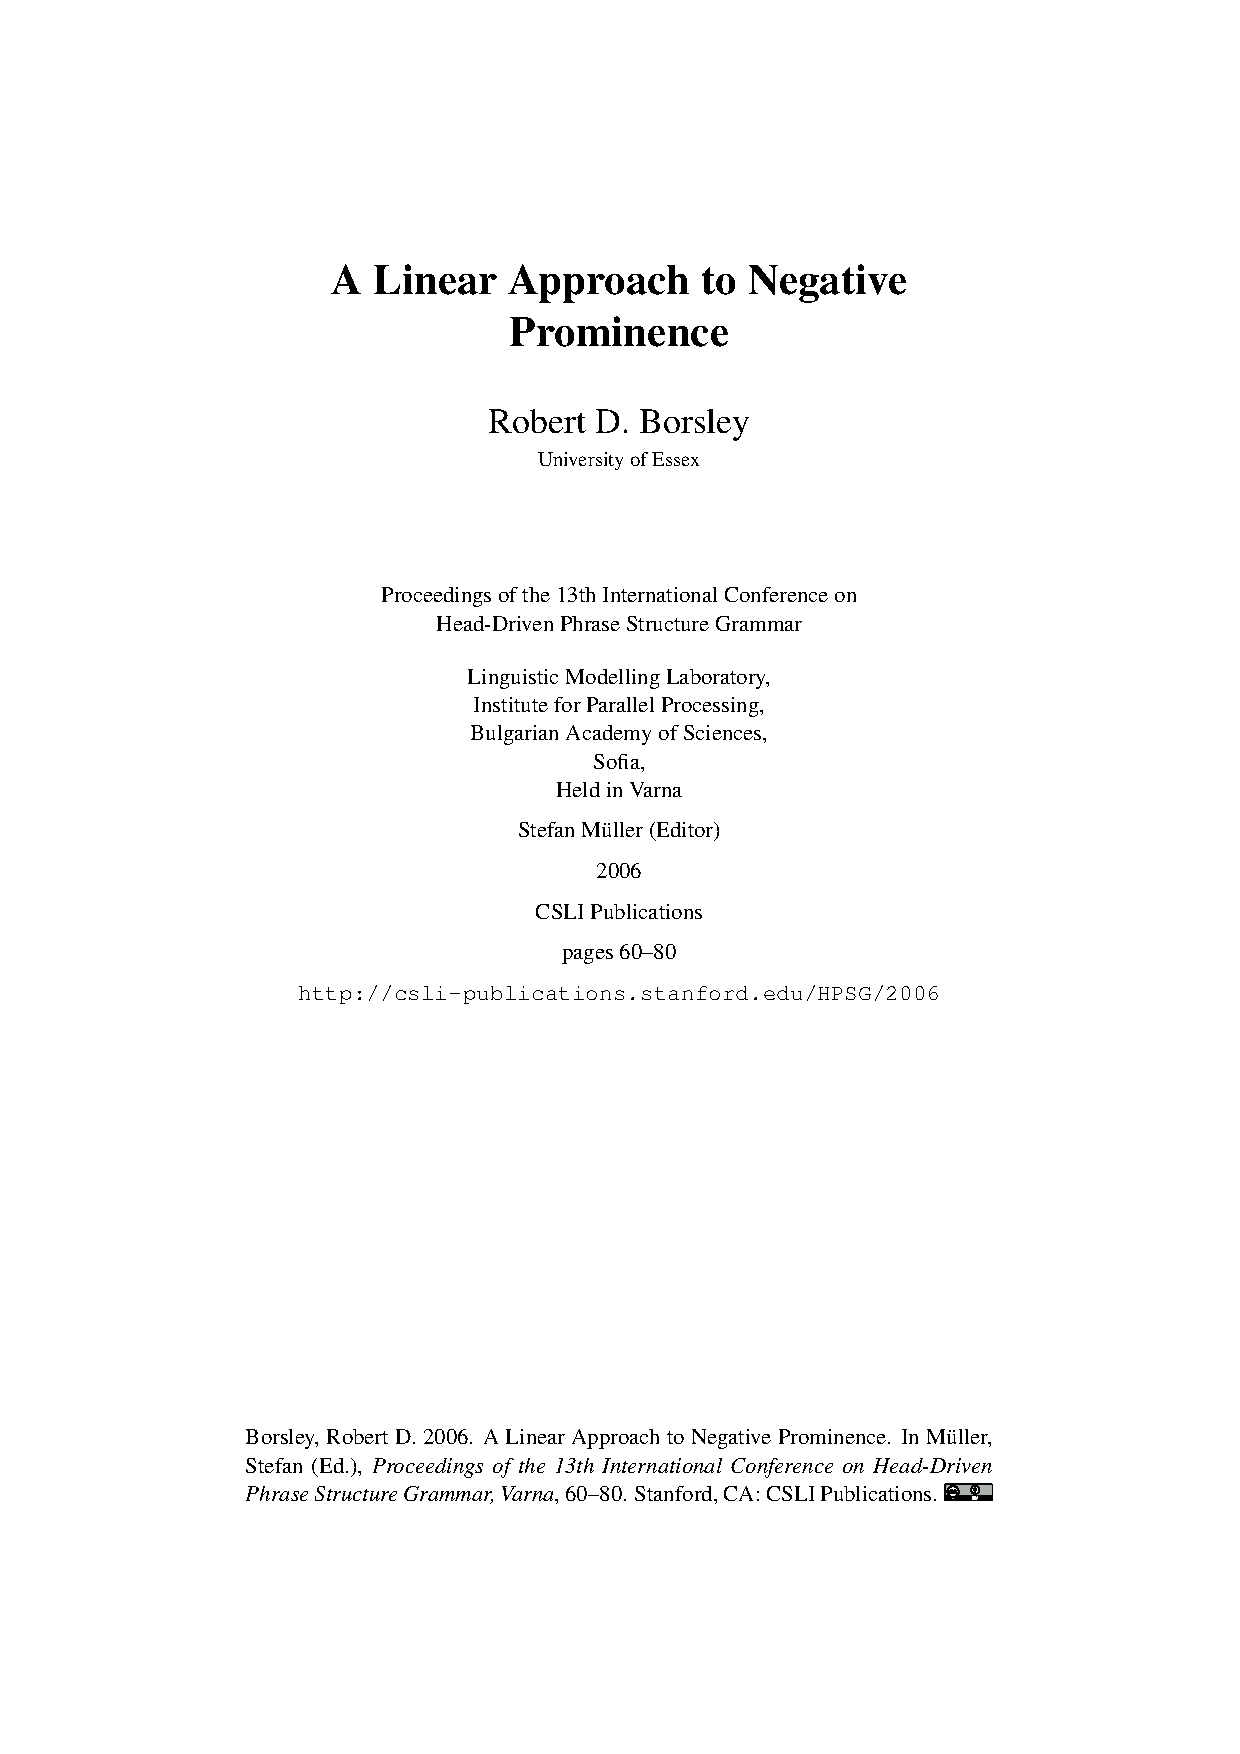
\includepdf[pages=-,pagecommand=\thispagestyle{plain},
            addtotoc={1,section,1,
            {Robert D. Borsley: A Linear Approach to Negative Prominence},
             borsley}]{borsley.pdf}

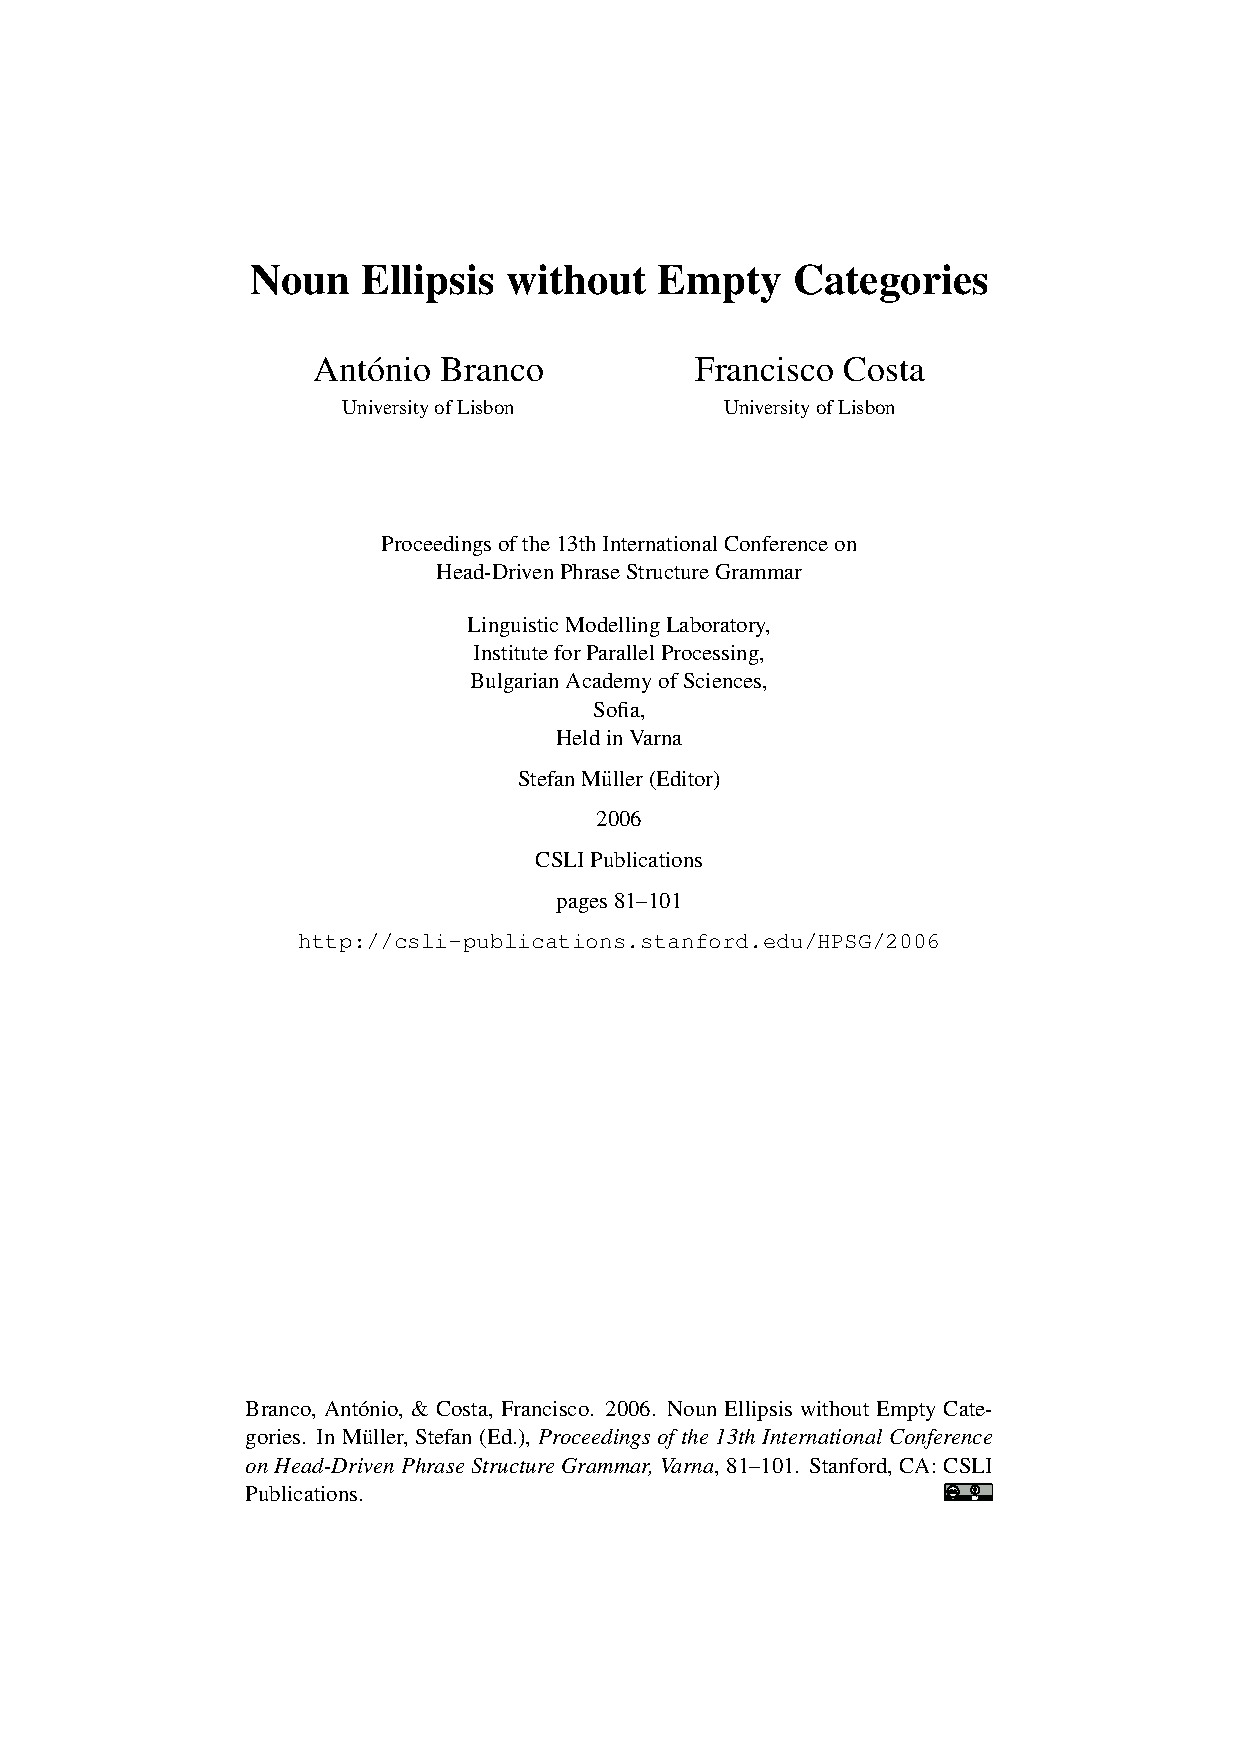
\includepdf[pages=-,pagecommand=\thispagestyle{plain},
            addtotoc={1,section,1,
            {Ant�nio Branco and Francisco Costa: Noun Ellipsis without Empty Categories},
             bc}]{branco-costa.pdf}


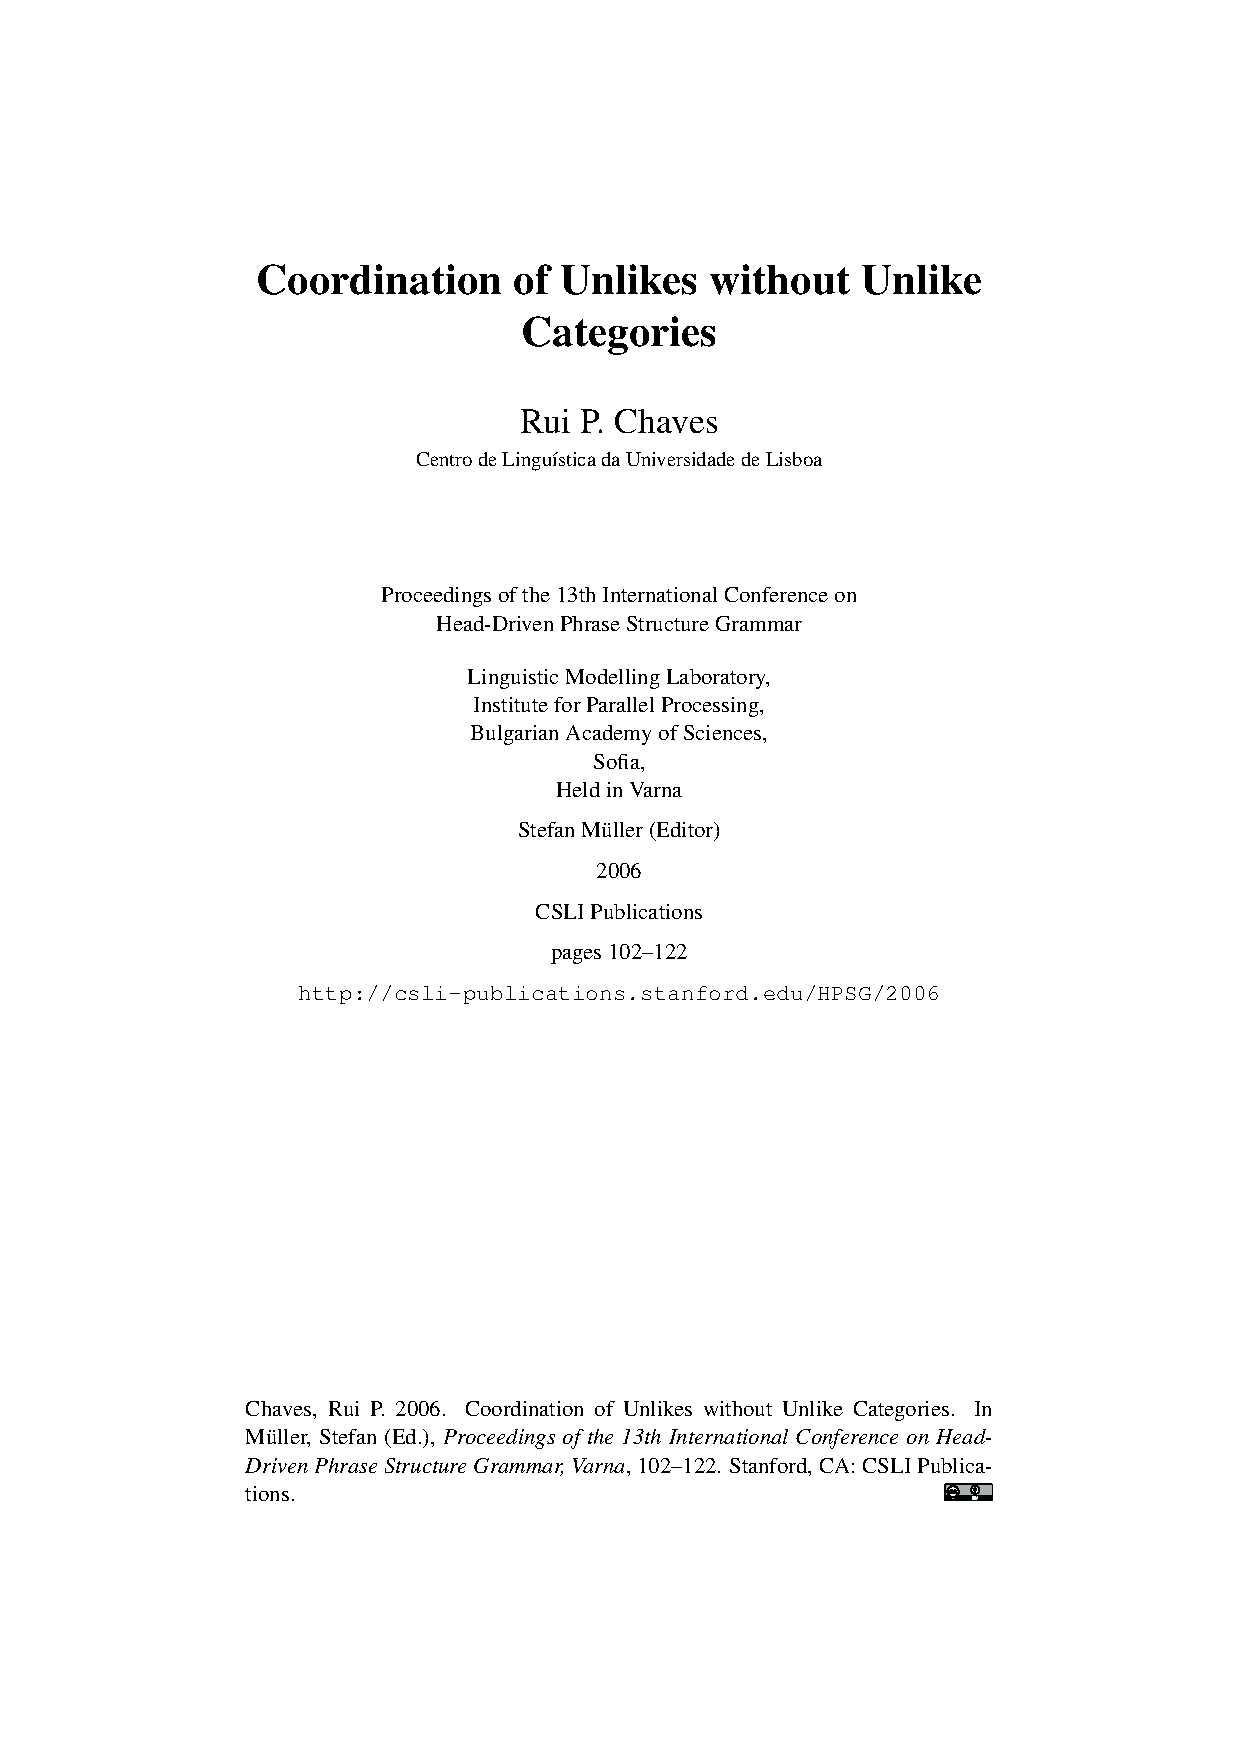
\includepdf[pages=-,pagecommand=\thispagestyle{plain},
            addtotoc={1,section,1,
            {Rui P. Chaves: Coordination of Unlikes without Unlike Categories},
             chaves}]{chaves.pdf}

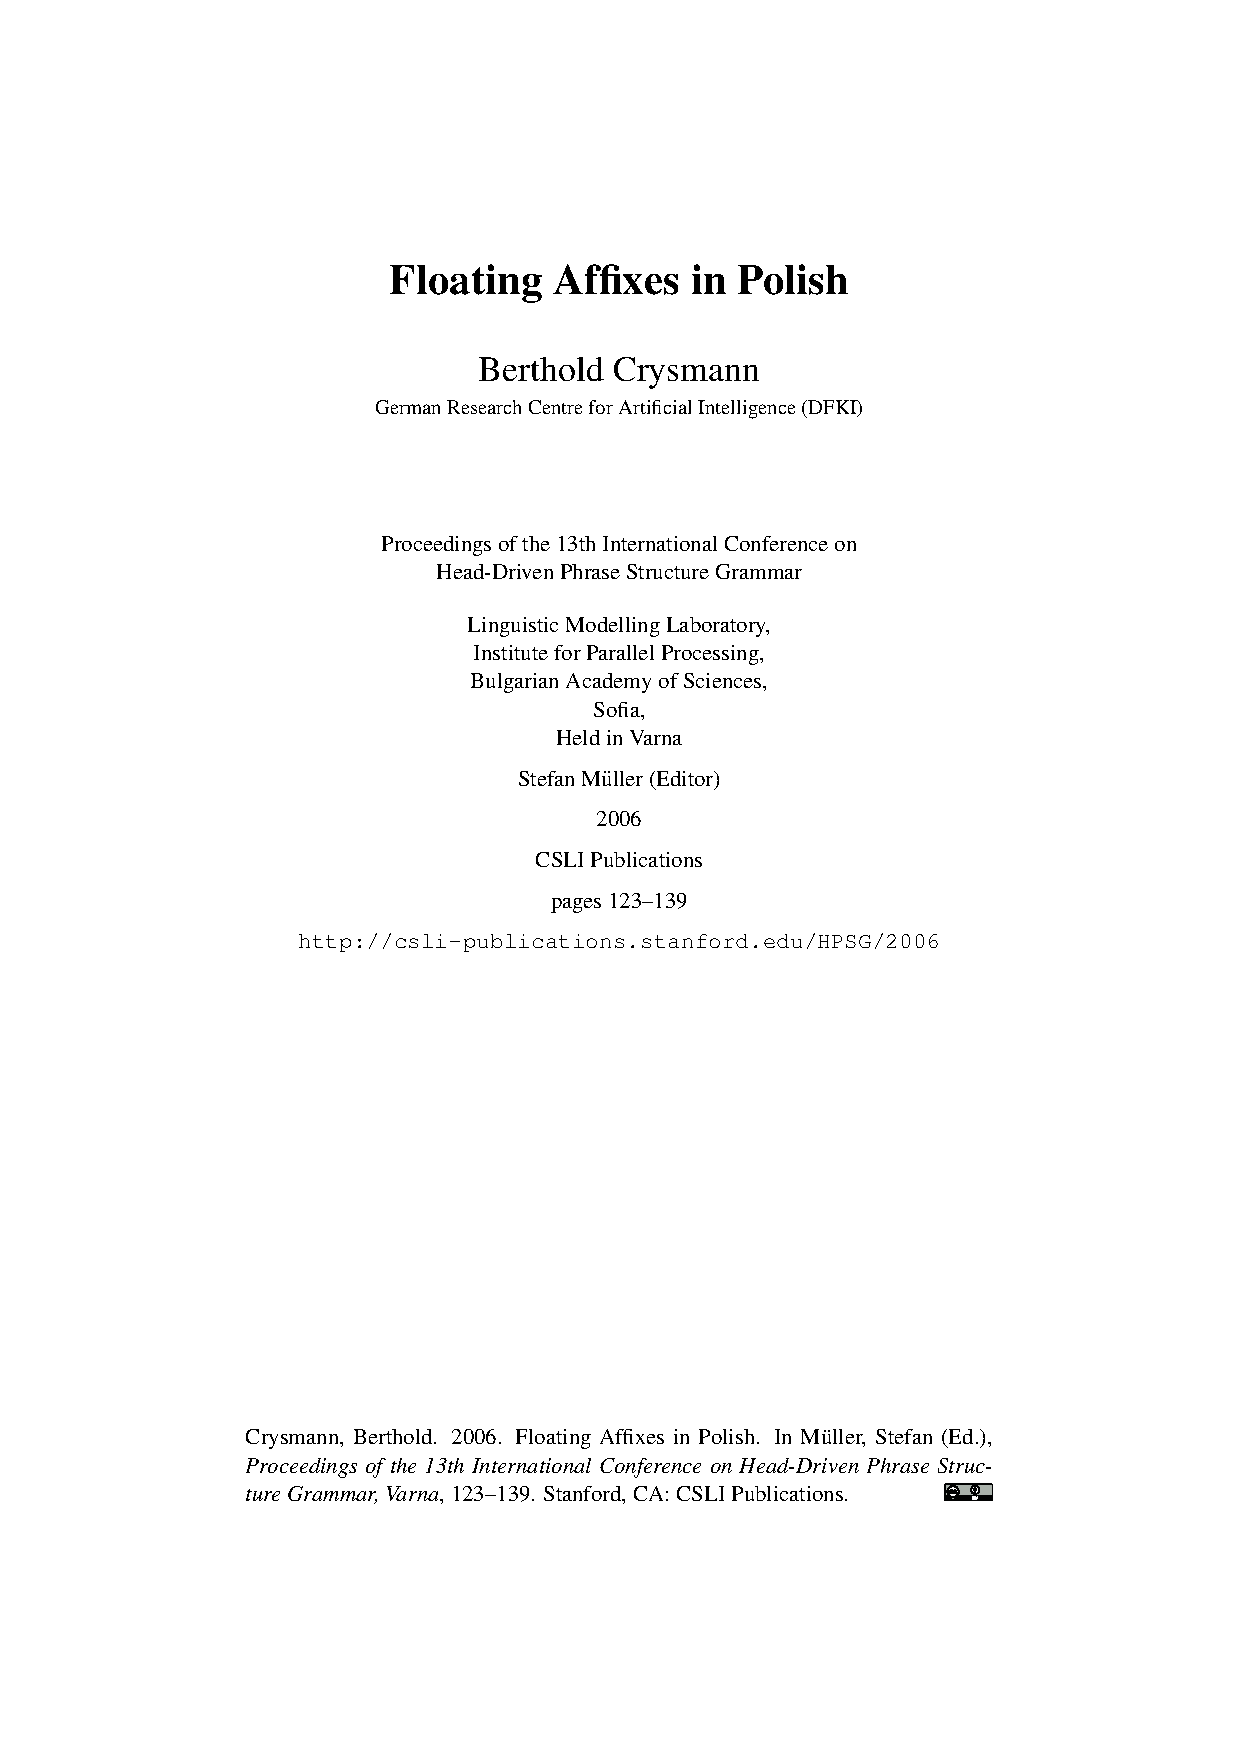
\includepdf[pages=-,pagecommand=\thispagestyle{plain},
            addtotoc={1,section,1,
            {Berthold Crysmann: Floating Affixes in Polish},
             crysmann}]{crysmann.pdf}


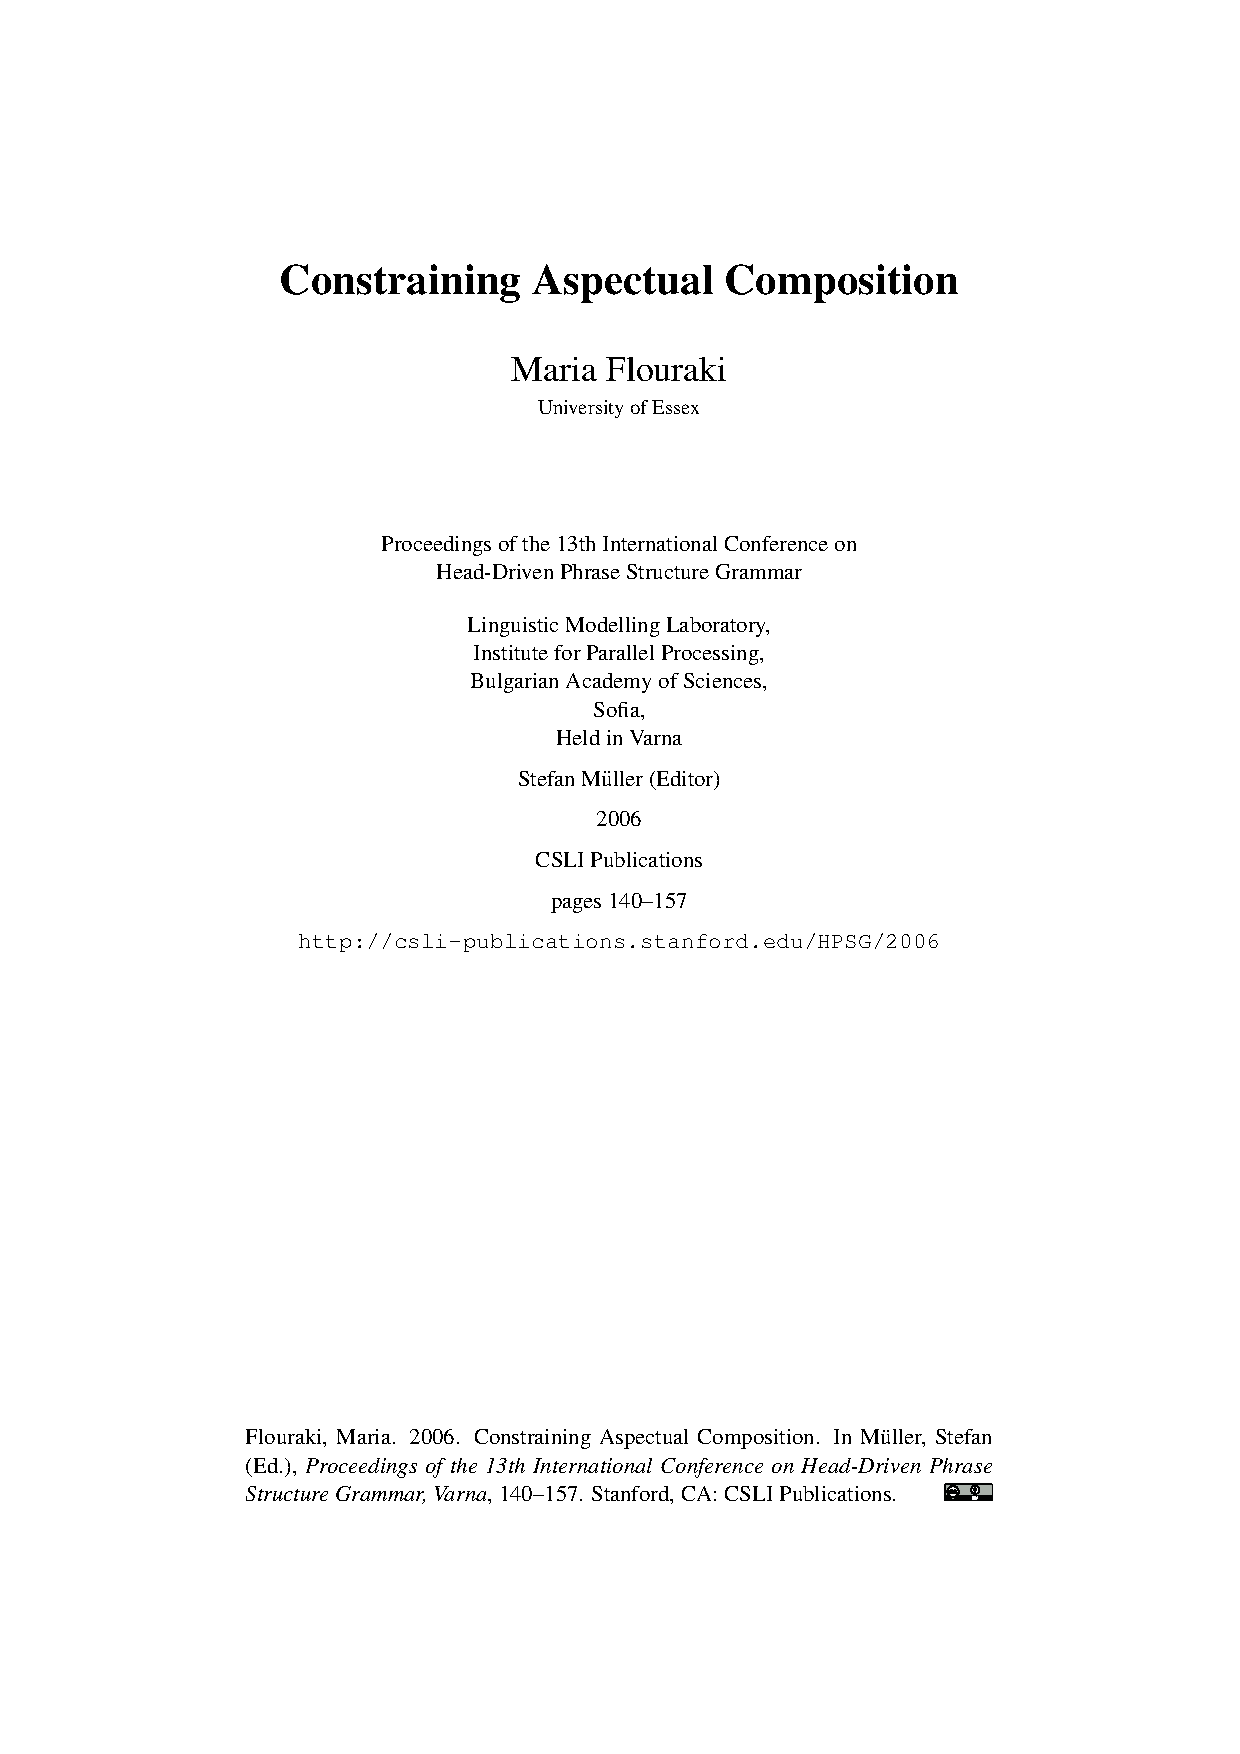
\includepdf[pages=-,pagecommand=\thispagestyle{plain},
            addtotoc={1,section,1,
            {Maria Flouraki: Constraining Aspectual Composition},
             flouraki}]{flouraki.pdf}

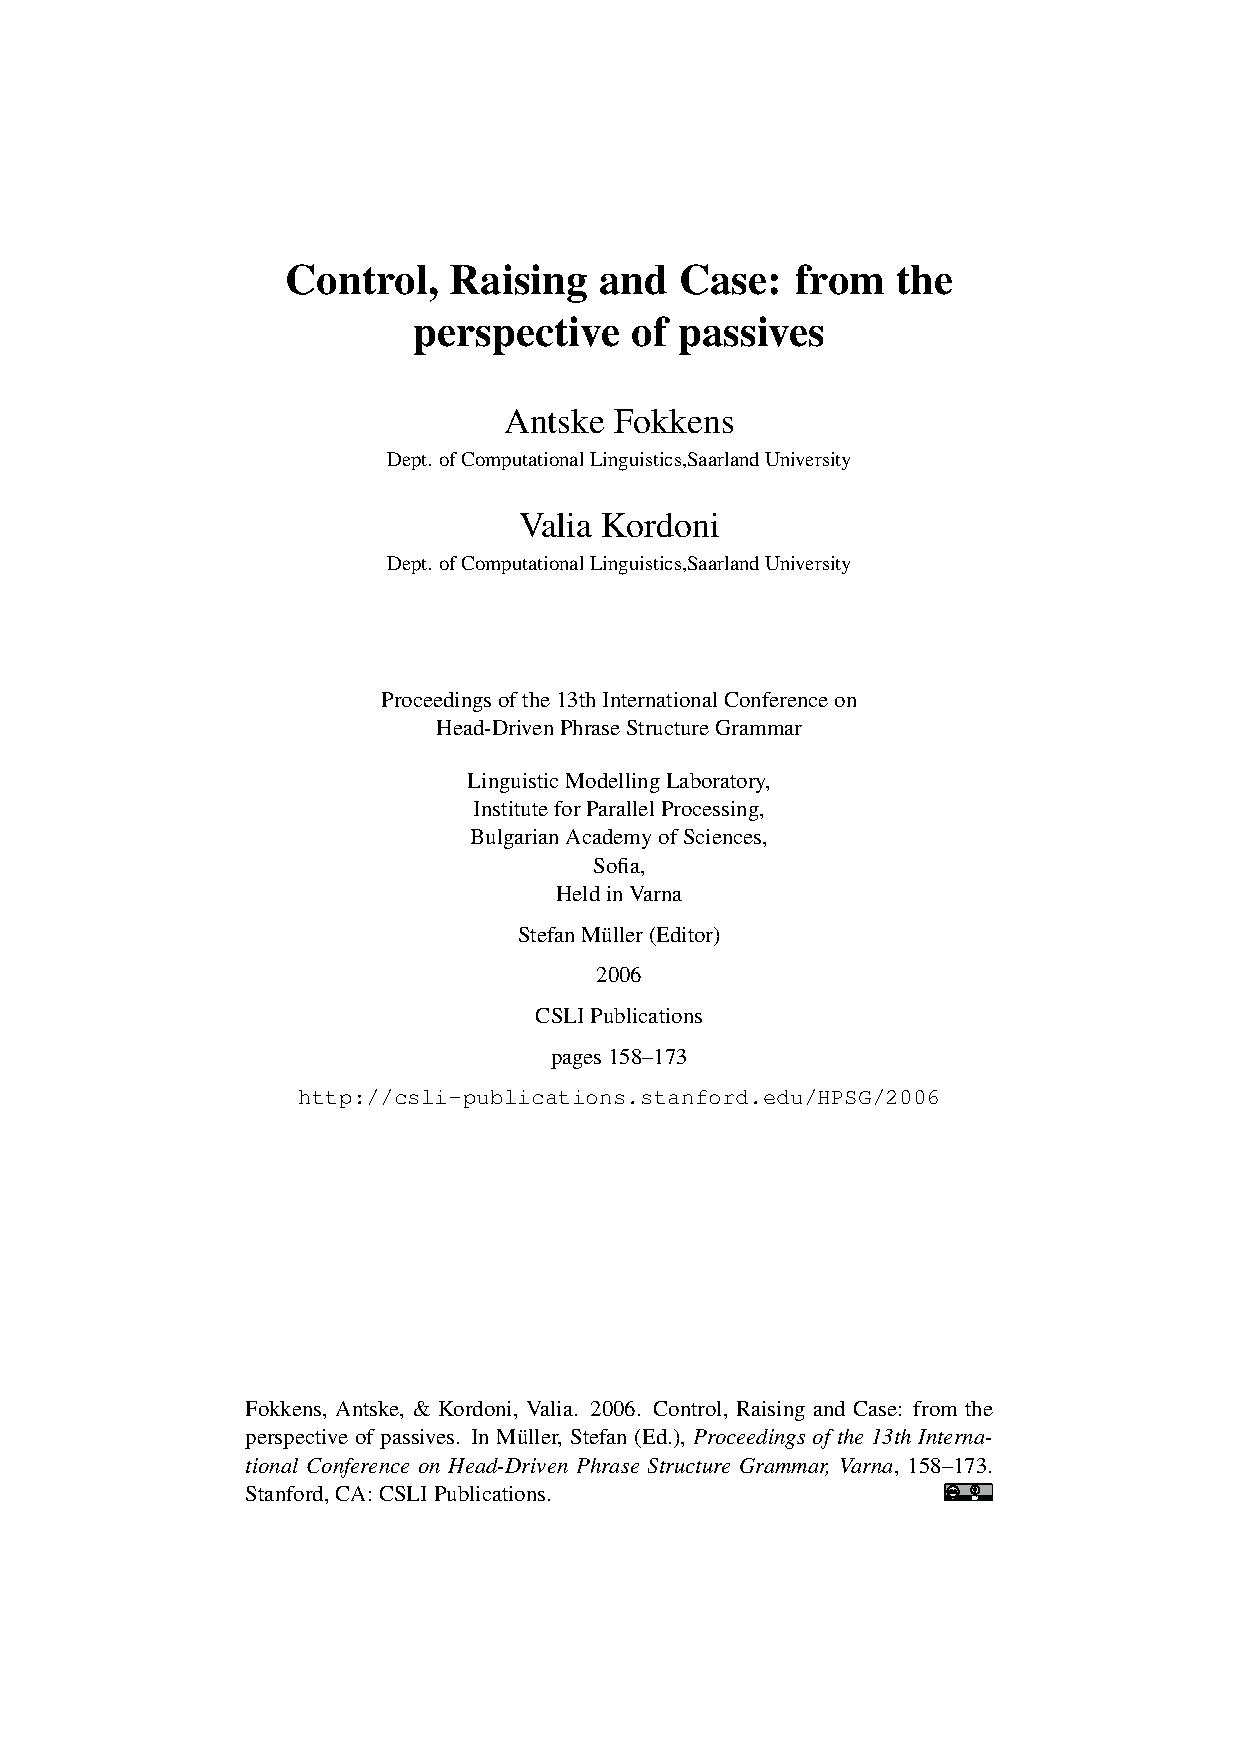
\includepdf[pages=-,pagecommand=\thispagestyle{plain},
            addtotoc={1,section,1,
            {Antske Fokkens and Valia Kordoni: Control, Raising and Case: from the Perspective of Passives},
             fk}]{fokkens-kordoni.pdf}

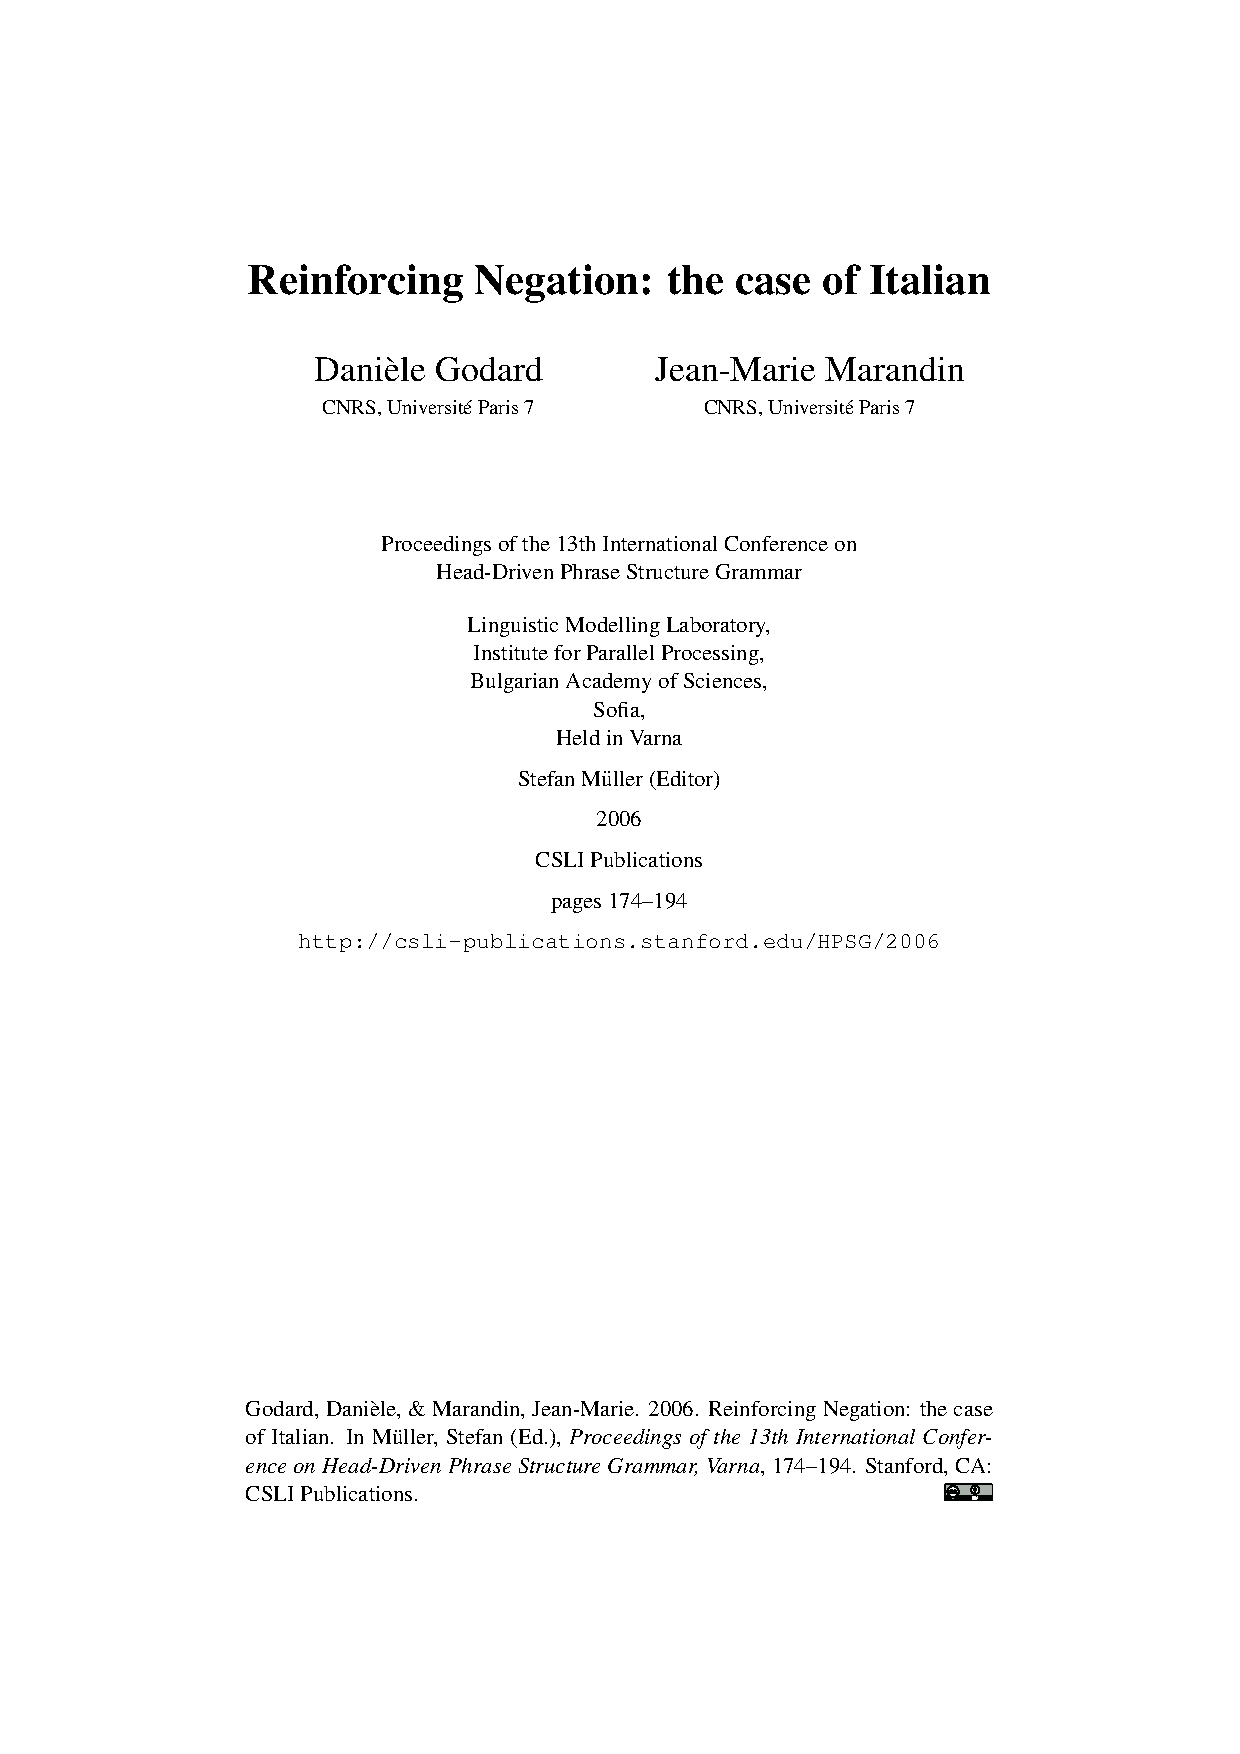
\includepdf[pages=-,pagecommand=\thispagestyle{plain},
            addtotoc={1,section,1,
            {Dani�le Godard and Jean-Marie Marandin: Reinforcing Negation: the Case of Italian},
             gm}]{godard-marandin.pdf}

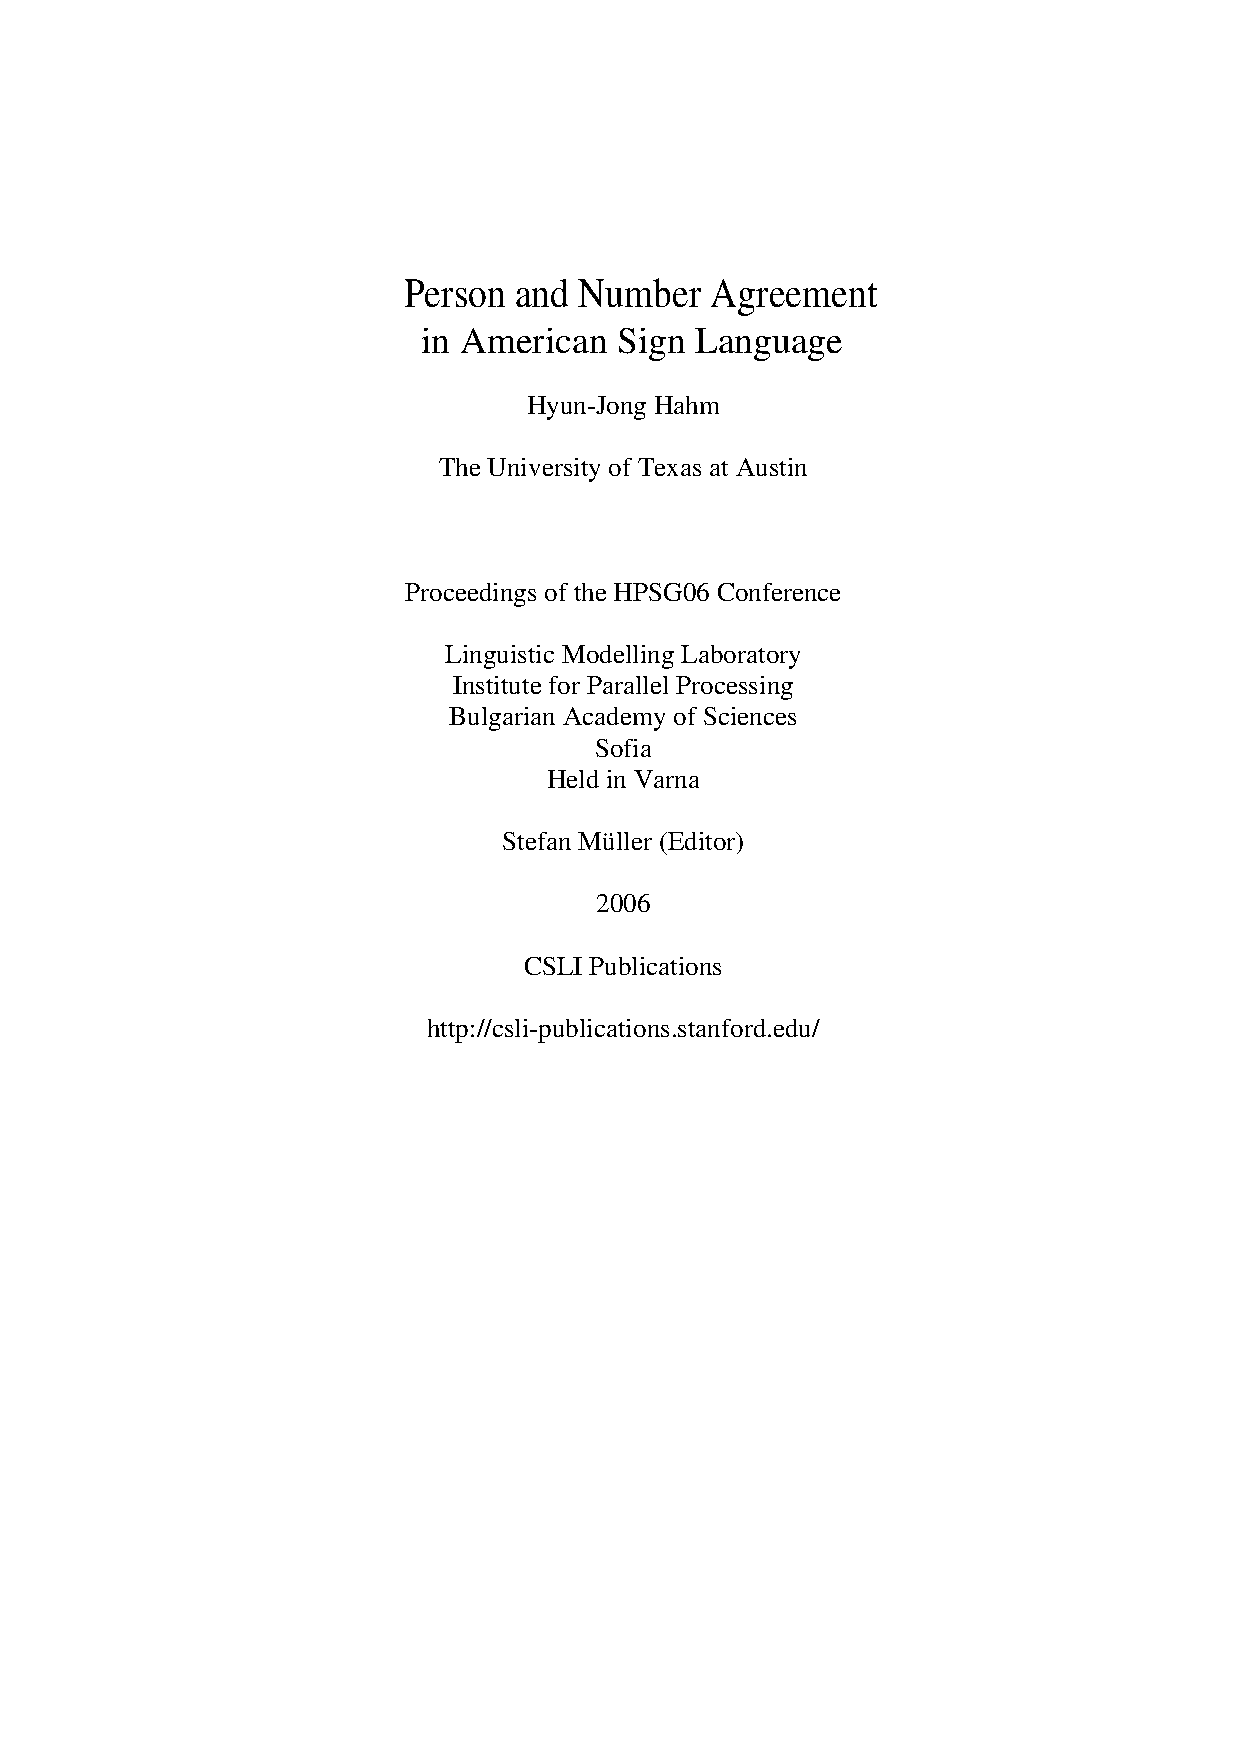
\includepdf[pages=-,pagecommand=\thispagestyle{plain},
            addtotoc={1,section,1,
            {Hyun-Jong Hahm: Person and Number Agreement in American Sign Language},
             hahm-asl}]{hahm-ASL.pdf}


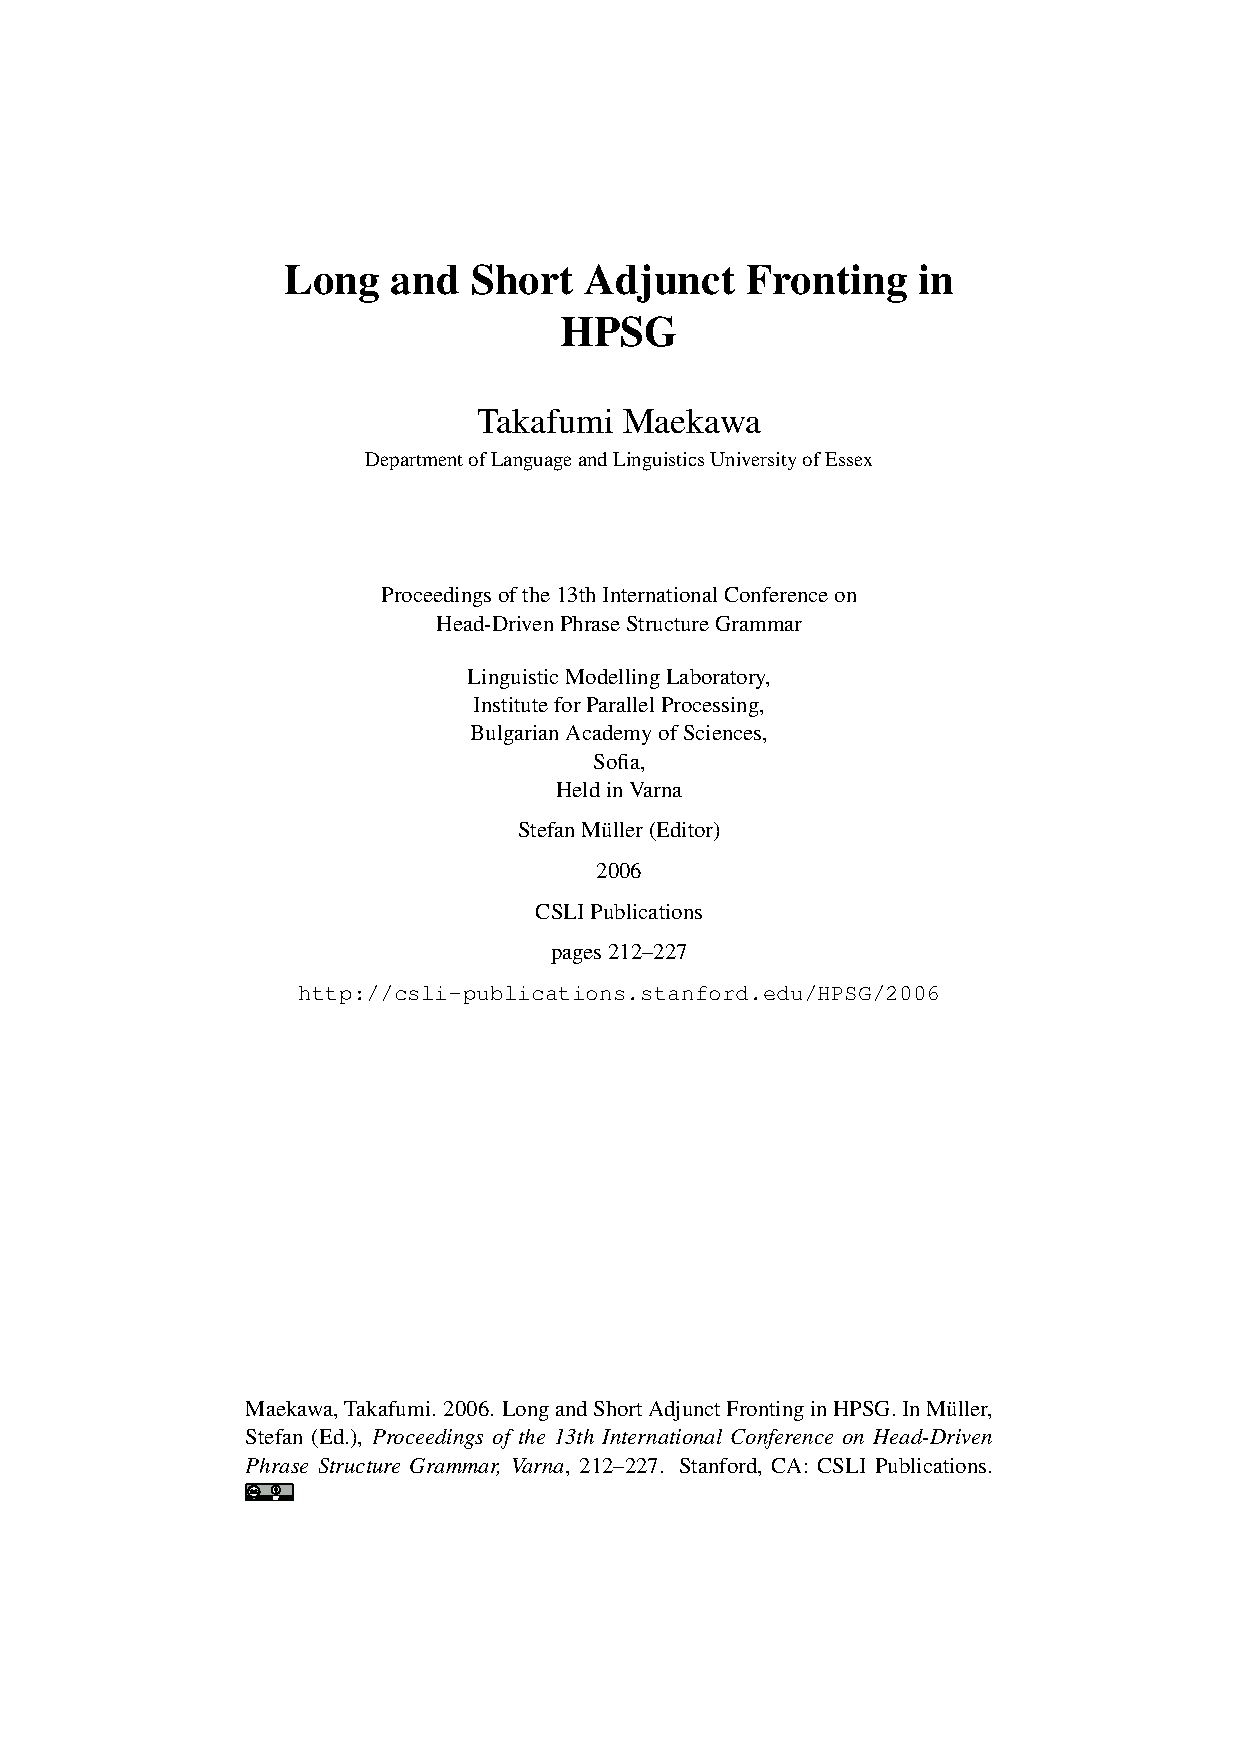
\includepdf[pages=-,pagecommand=\thispagestyle{plain},
            addtotoc={1,section,1,
            {Takafumi Maekawa: Long and Short Adjunct Fronting in HPSG},
             maekawa}]{maekawa.pdf}

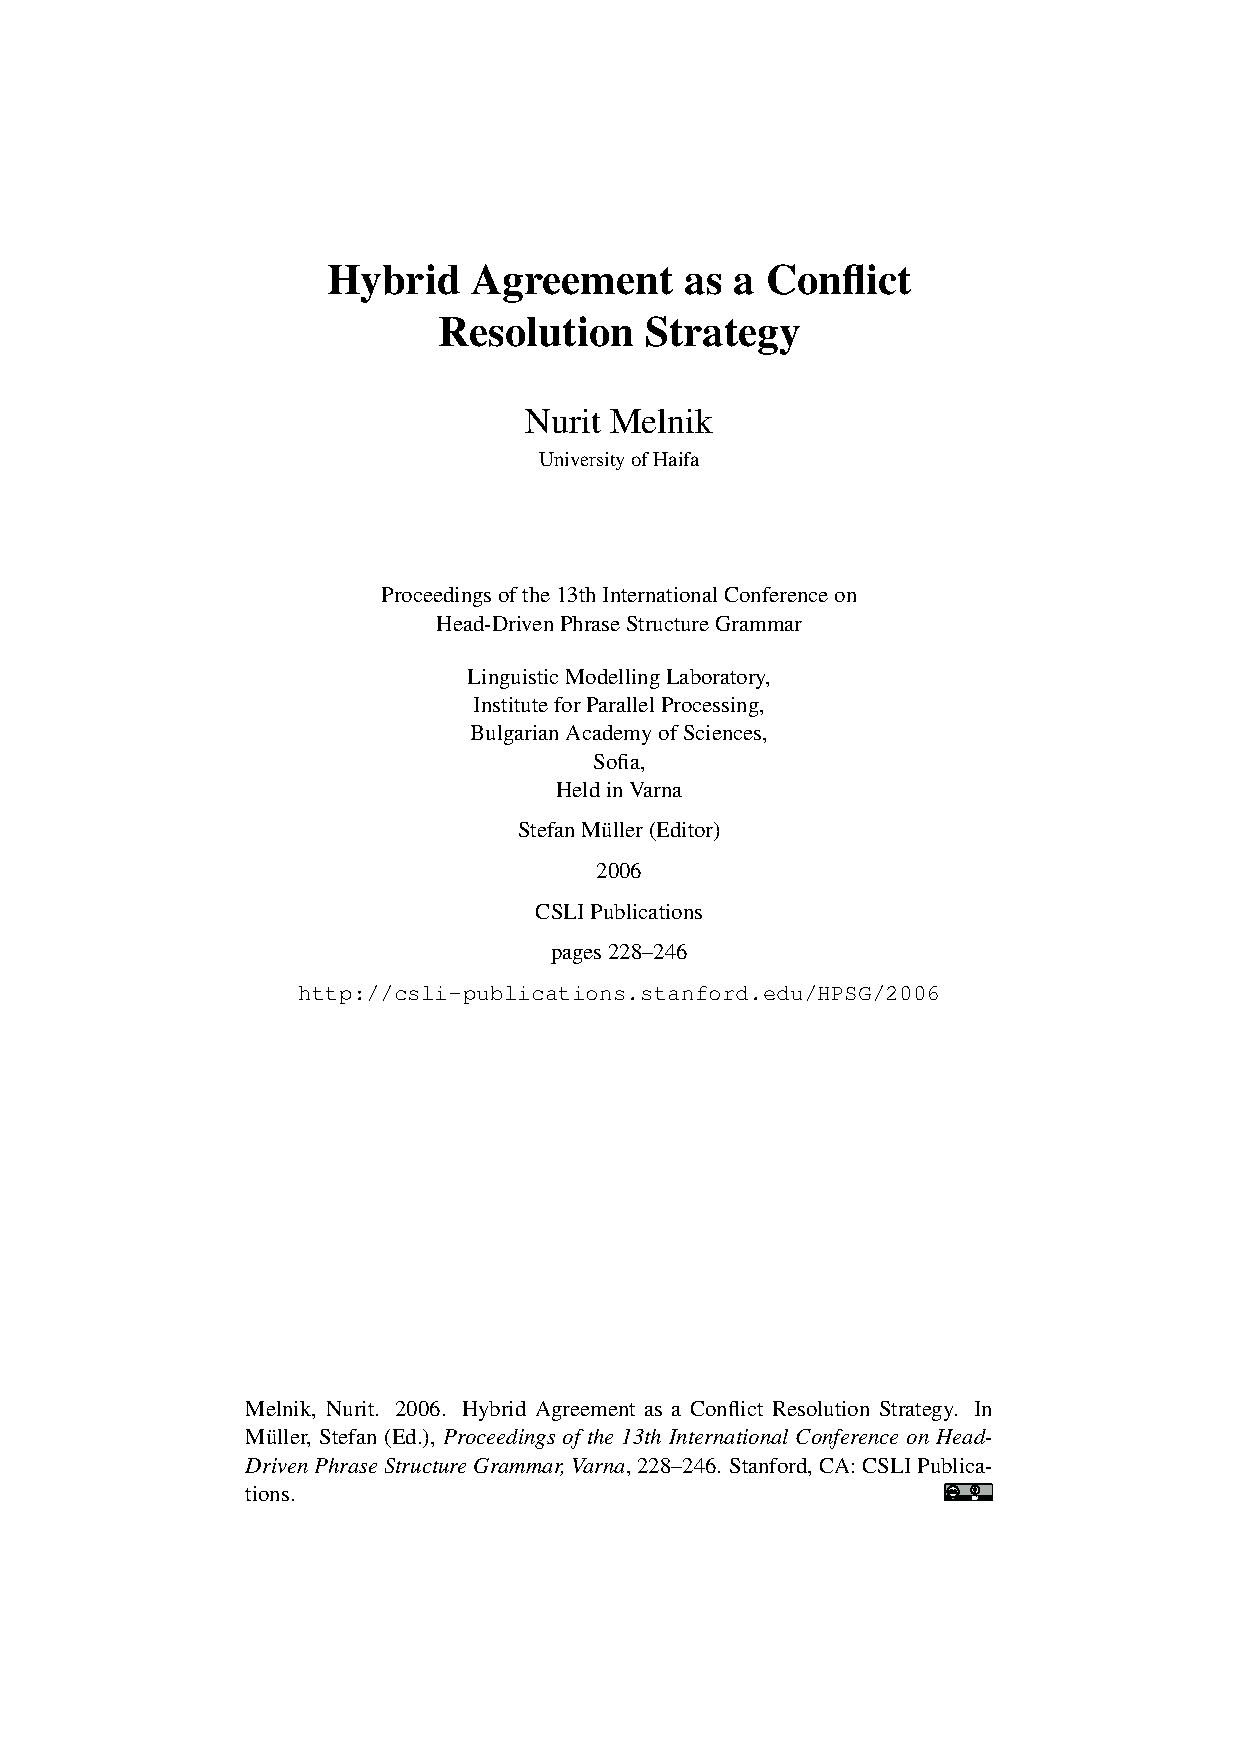
\includepdf[pages=-,pagecommand=\thispagestyle{plain},
            addtotoc={1,section,1,
            {Nurit Melnik: Hybrid Agreement as a Conflict Resolution Strategy},
             melnik}]{melnik.pdf}


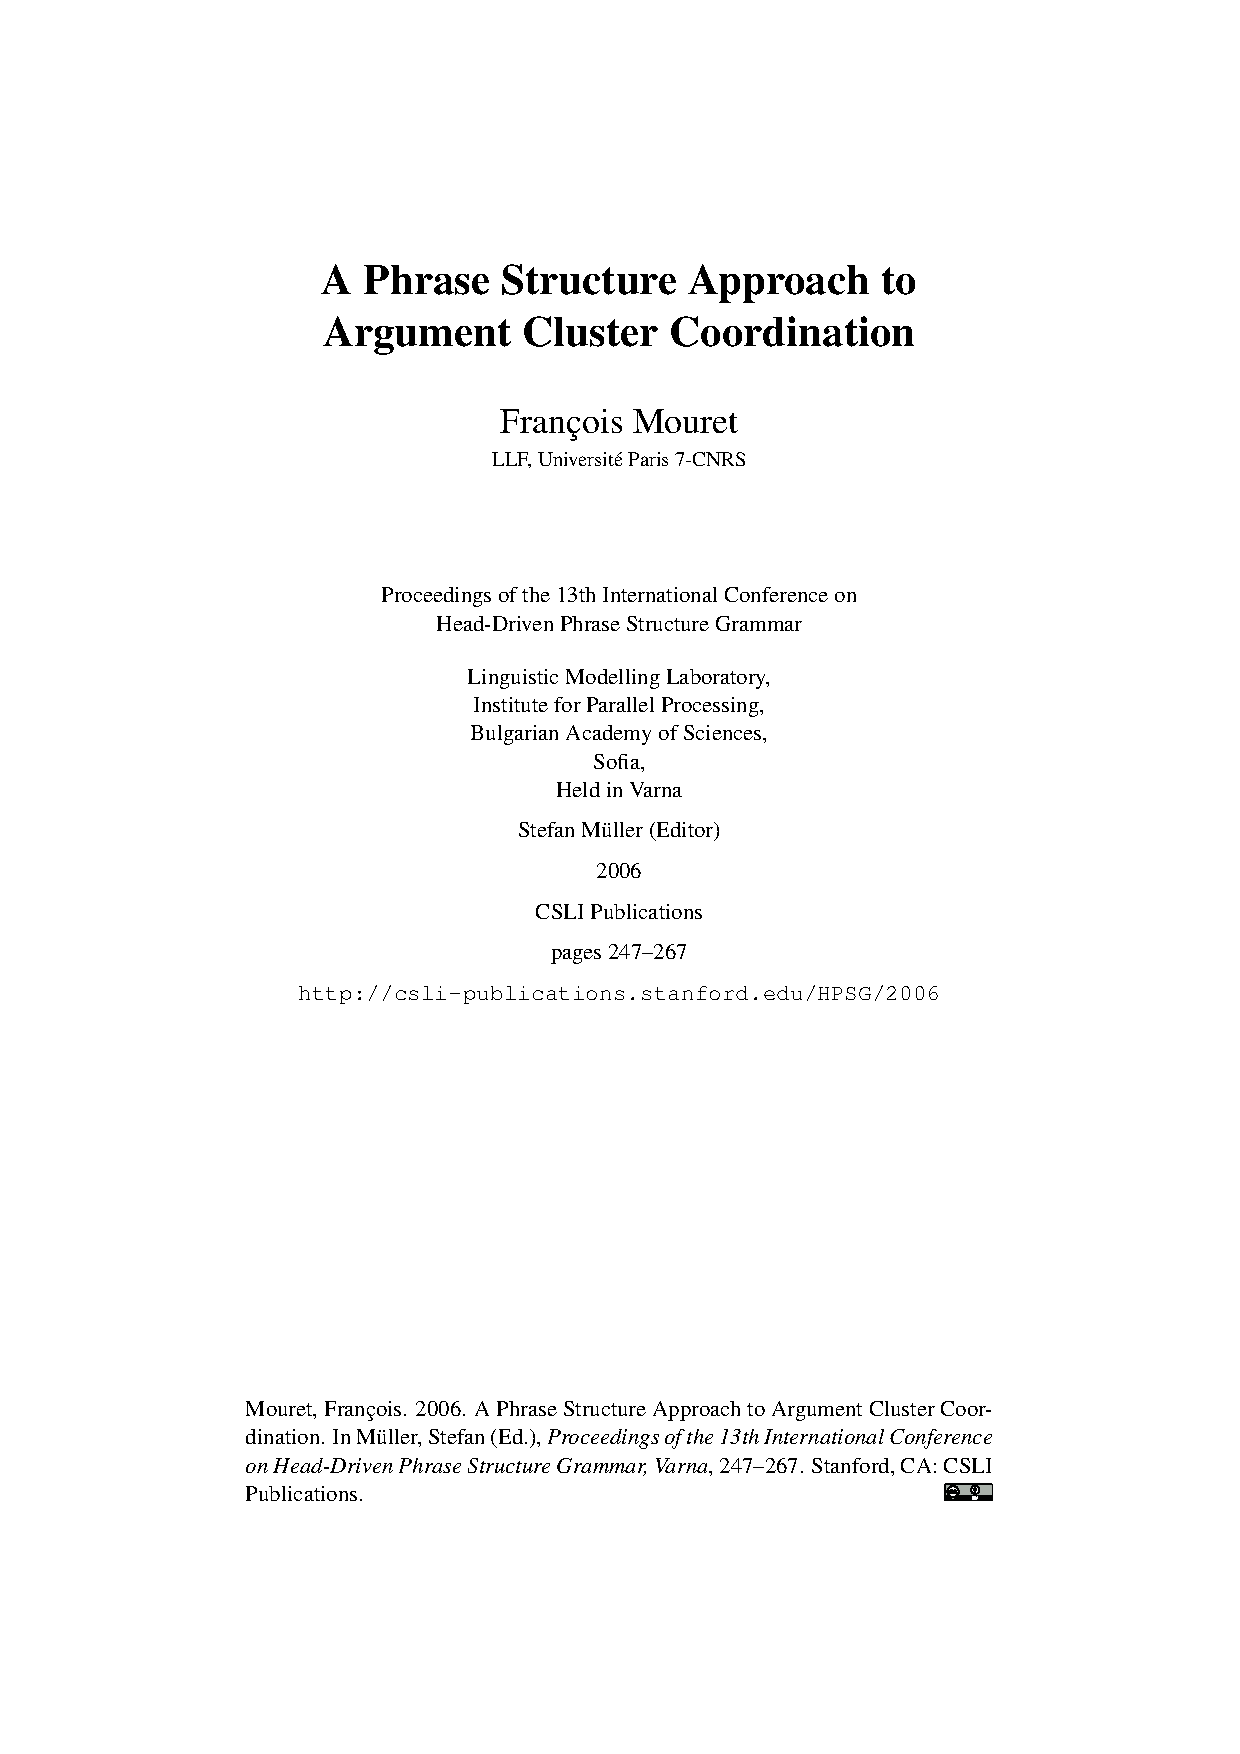
\includepdf[pages=-,pagecommand=\thispagestyle{plain},
            addtotoc={1,section,1,
            {Fran�ois Mouret: A Phrase Structure Approach to Argument Cluster Coordination},
             mouret}]{mouret.pdf}


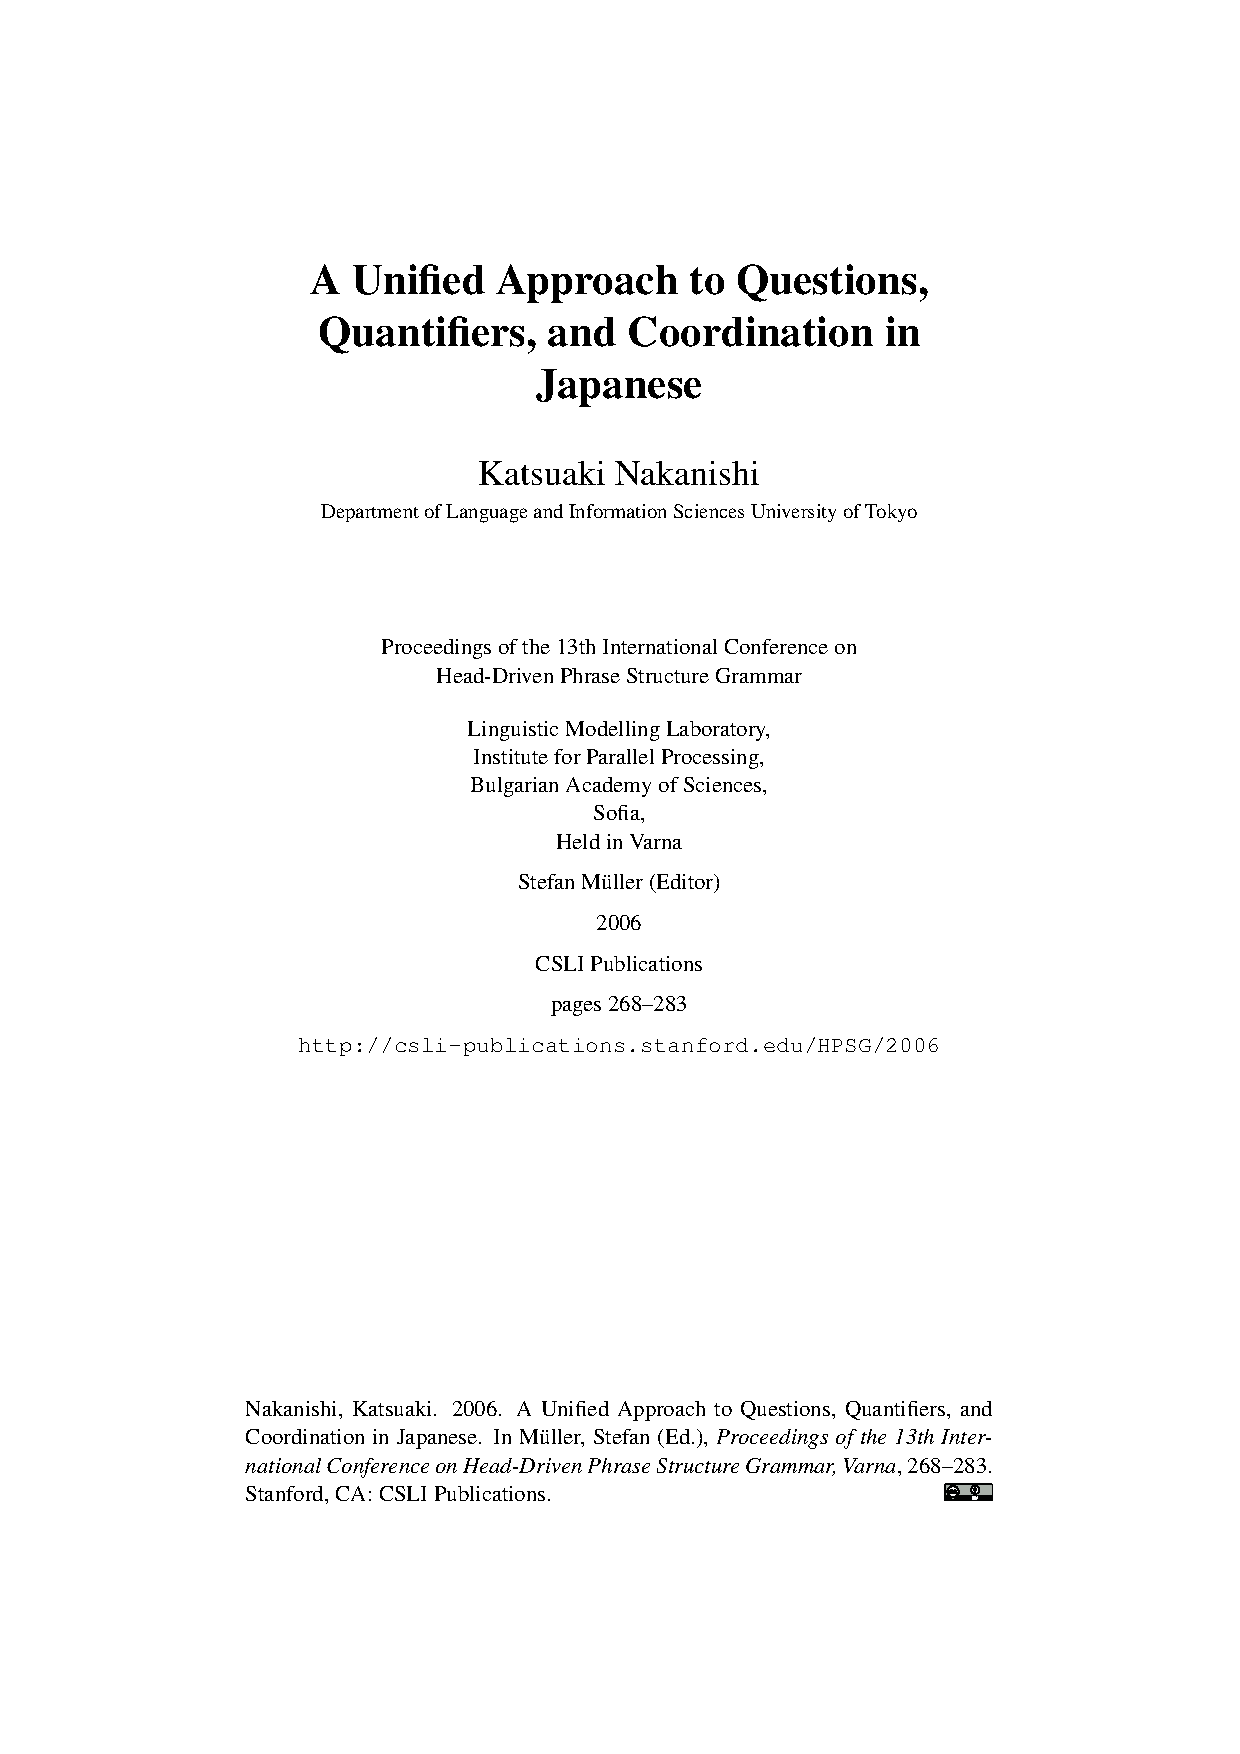
\includepdf[pages=-,pagecommand=\thispagestyle{plain},
            addtotoc={1,section,1,
            {Katsuaki Nakanishi: A Unified Approach to Questions, Quantifiers, and Coordination in Japanese},
             nakanishi}]{nakanishi.pdf}


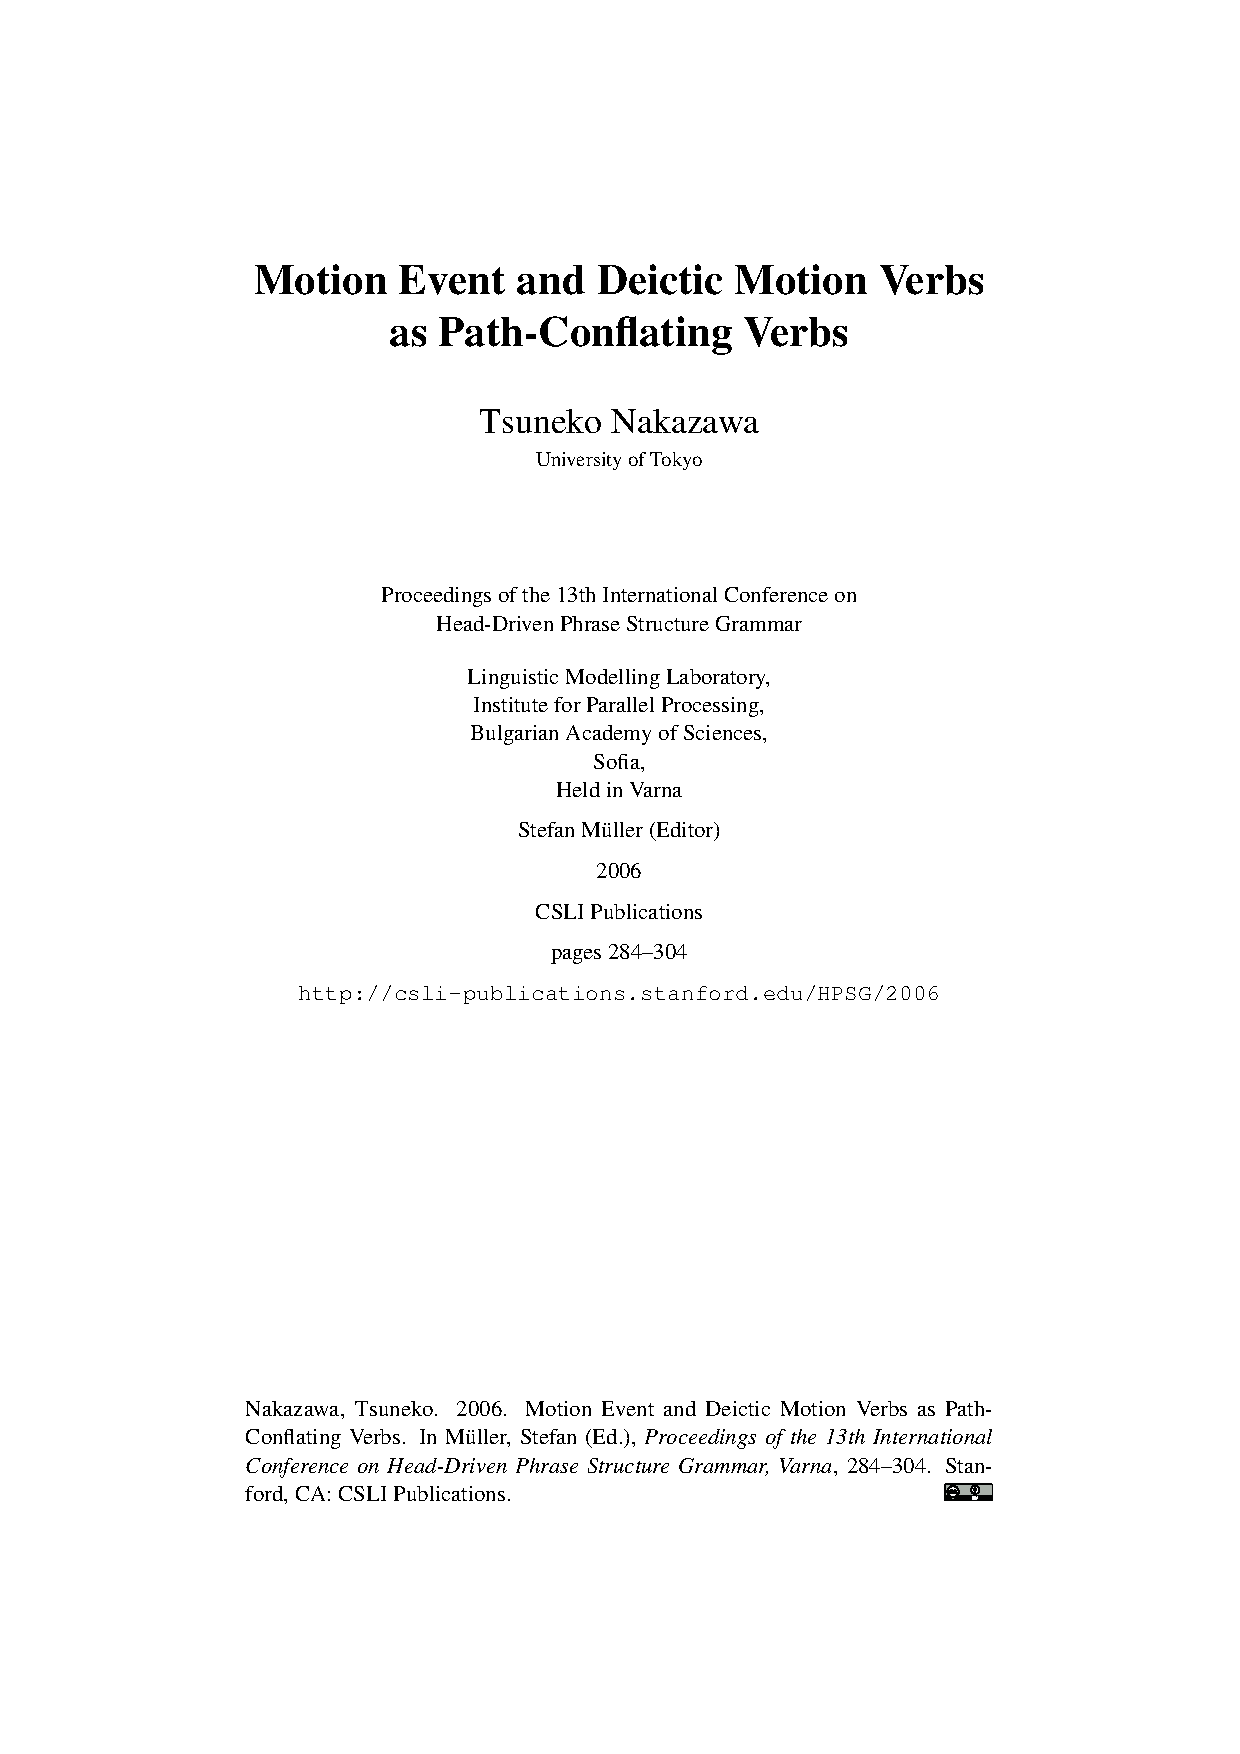
\includepdf[pages=-,pagecommand=\thispagestyle{plain},
            addtotoc={1,section,1,
            {Tsuneko Nakazawa: Motion Event and Deictic Motion Verbs as Path-Conflating Verbs},
             nakazawa}]{nakazawa.pdf}

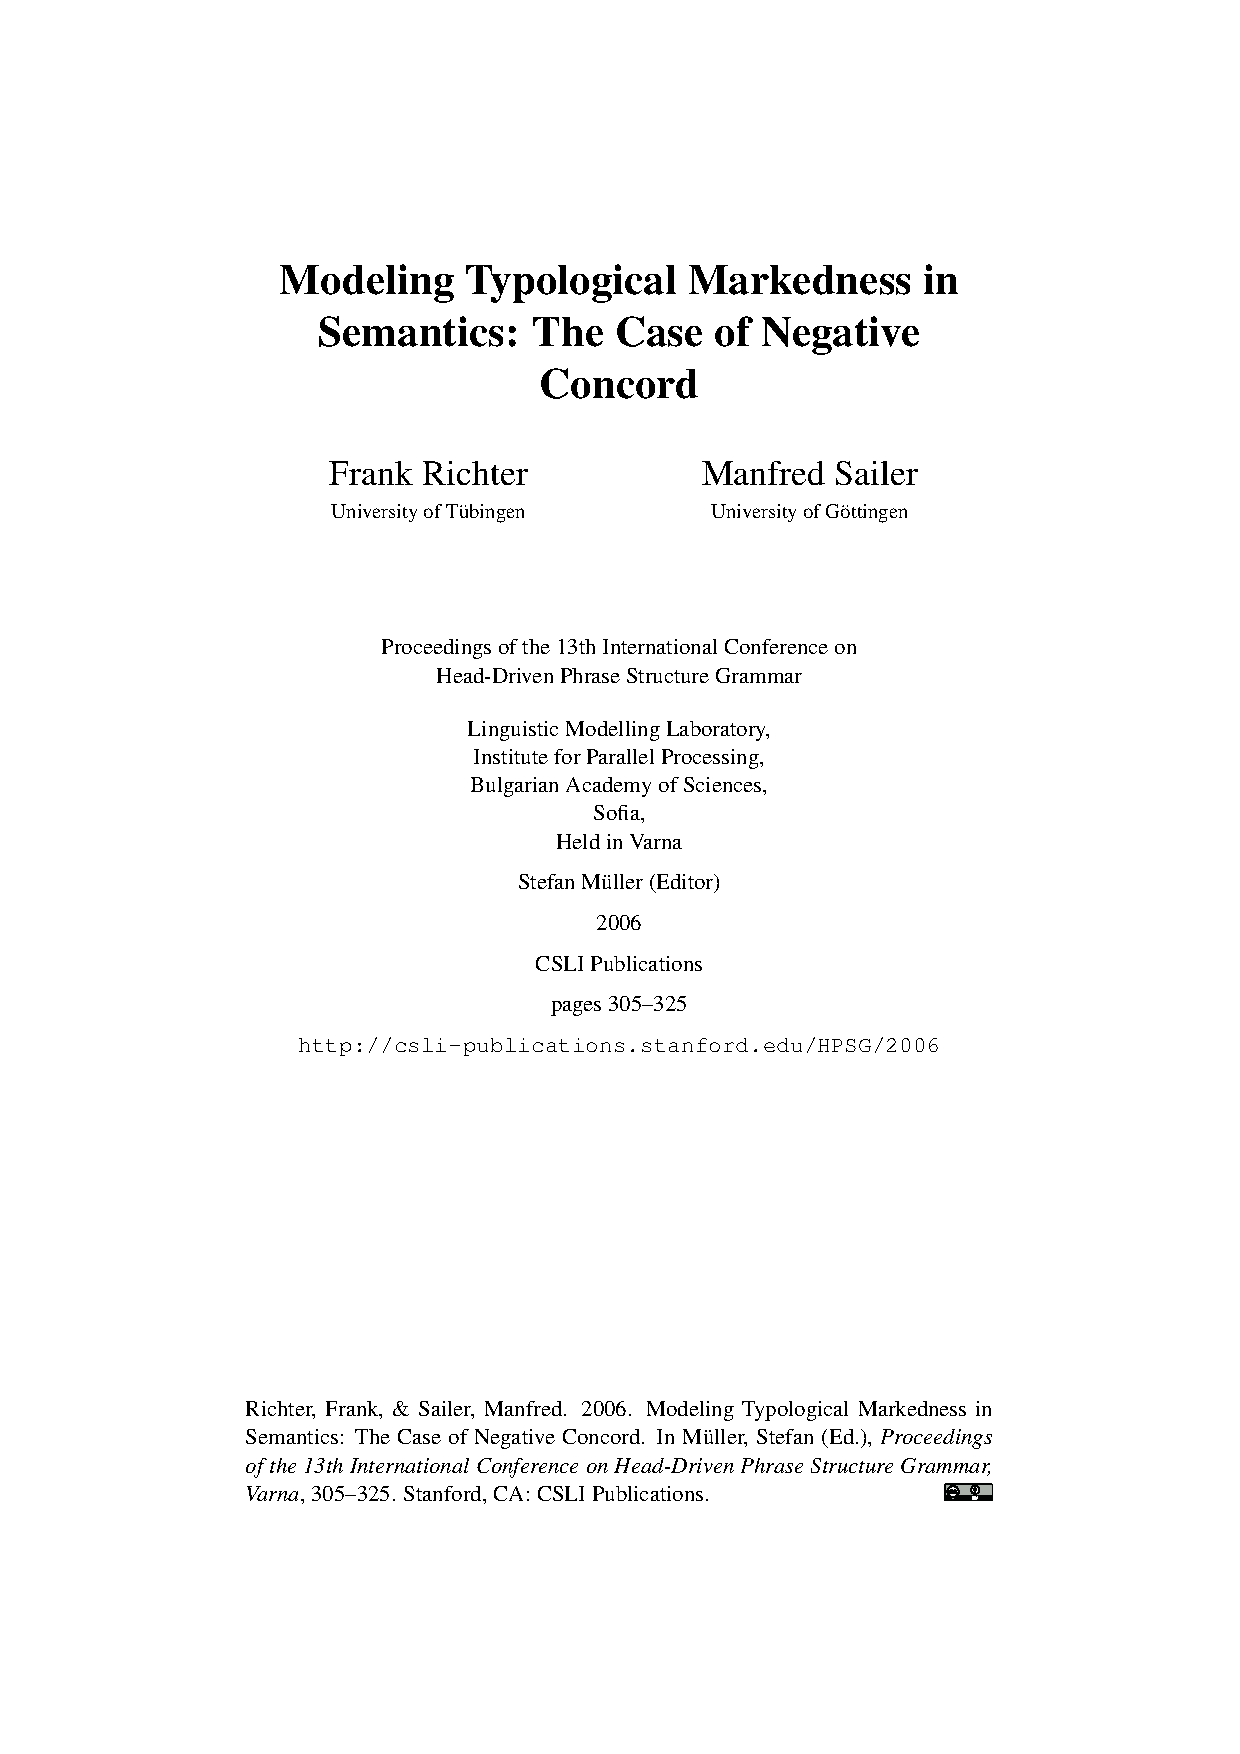
\includepdf[pages=-,pagecommand=\thispagestyle{plain},
            addtotoc={1,section,1,
            {Frank Richter and Manfred Sailer: Modeling Typological Markedness in Semantics: The Case of Negative Concord},
             rs}]{richter-sailer.pdf}


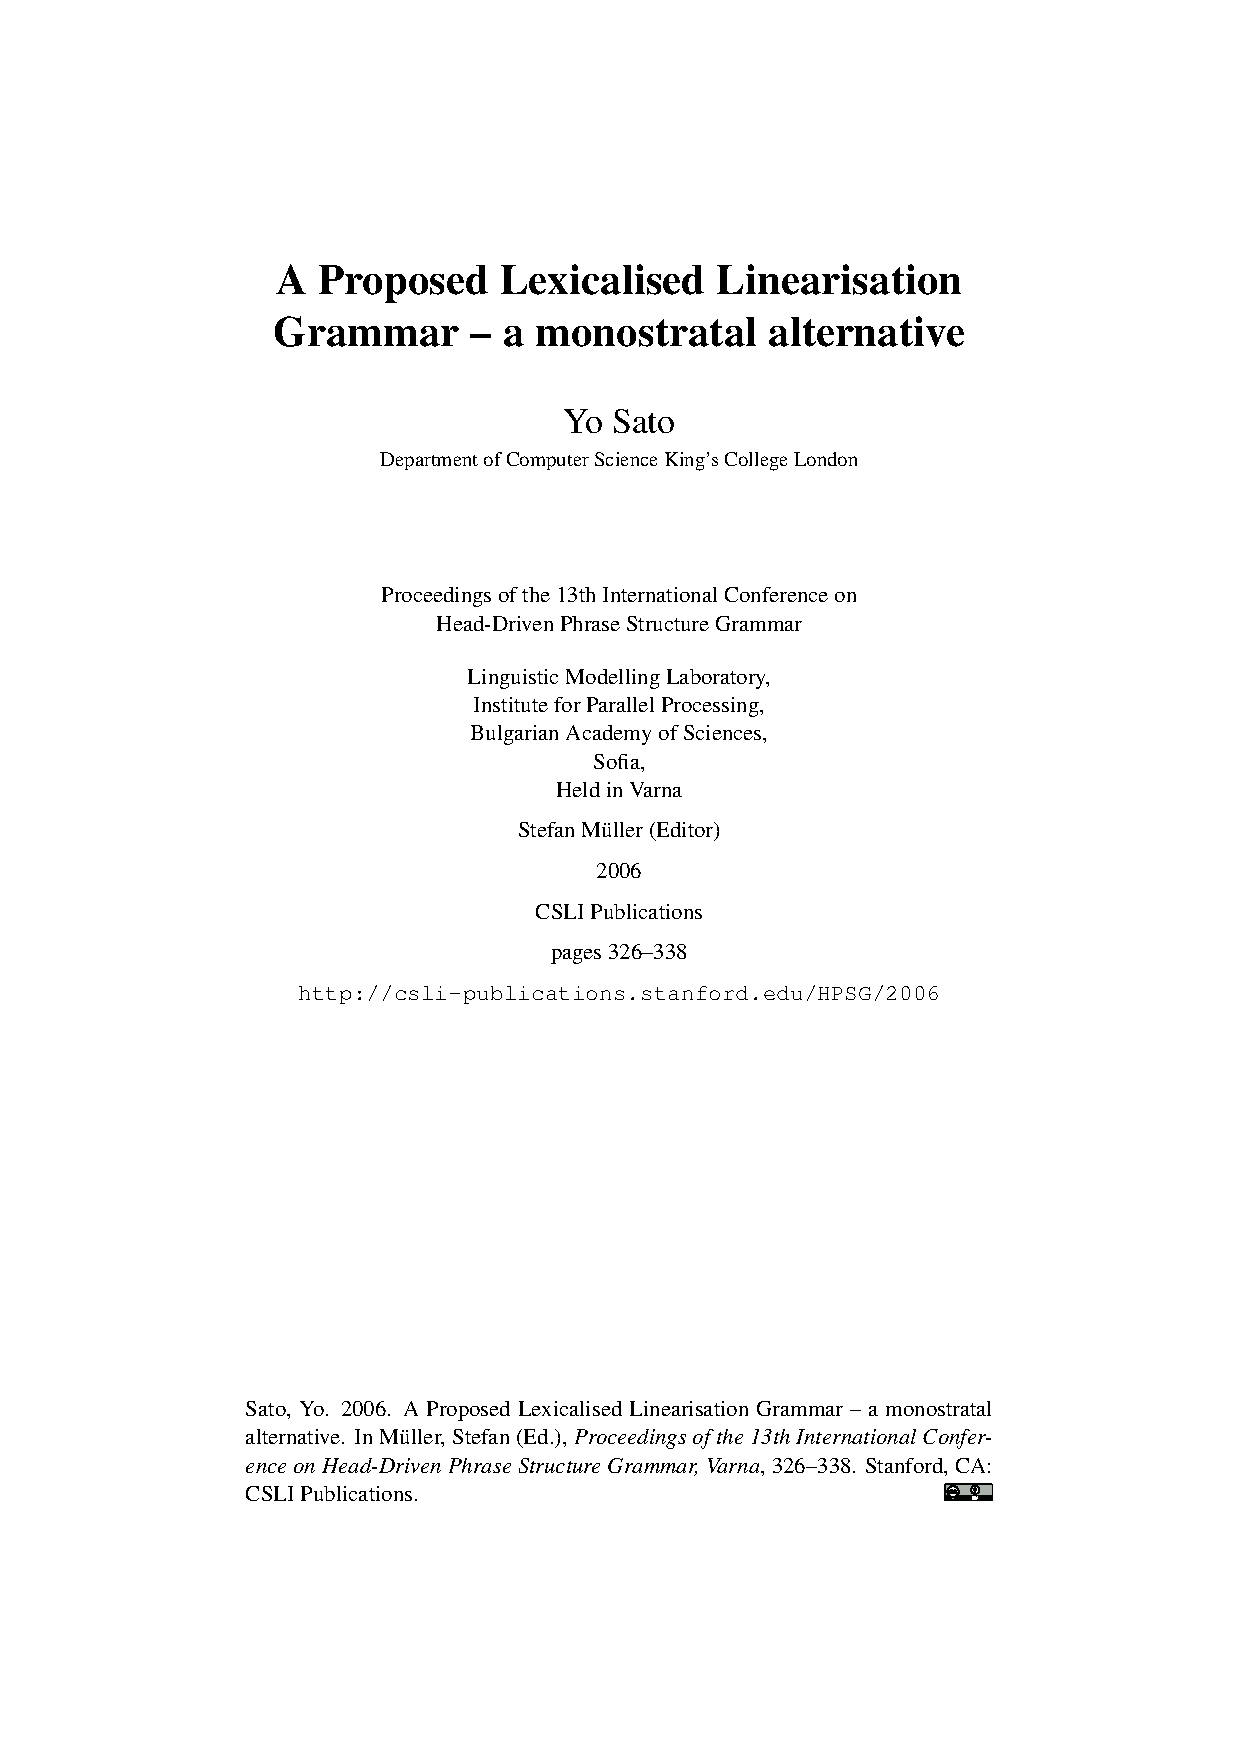
\includepdf[pages=-,pagecommand=\thispagestyle{plain},
            addtotoc={1,section,1,
            {Yo Sato: A Proposed Lexicalised Linearisation Grammar -- a Monostratal Alternative},
             sato}]{sato.pdf}

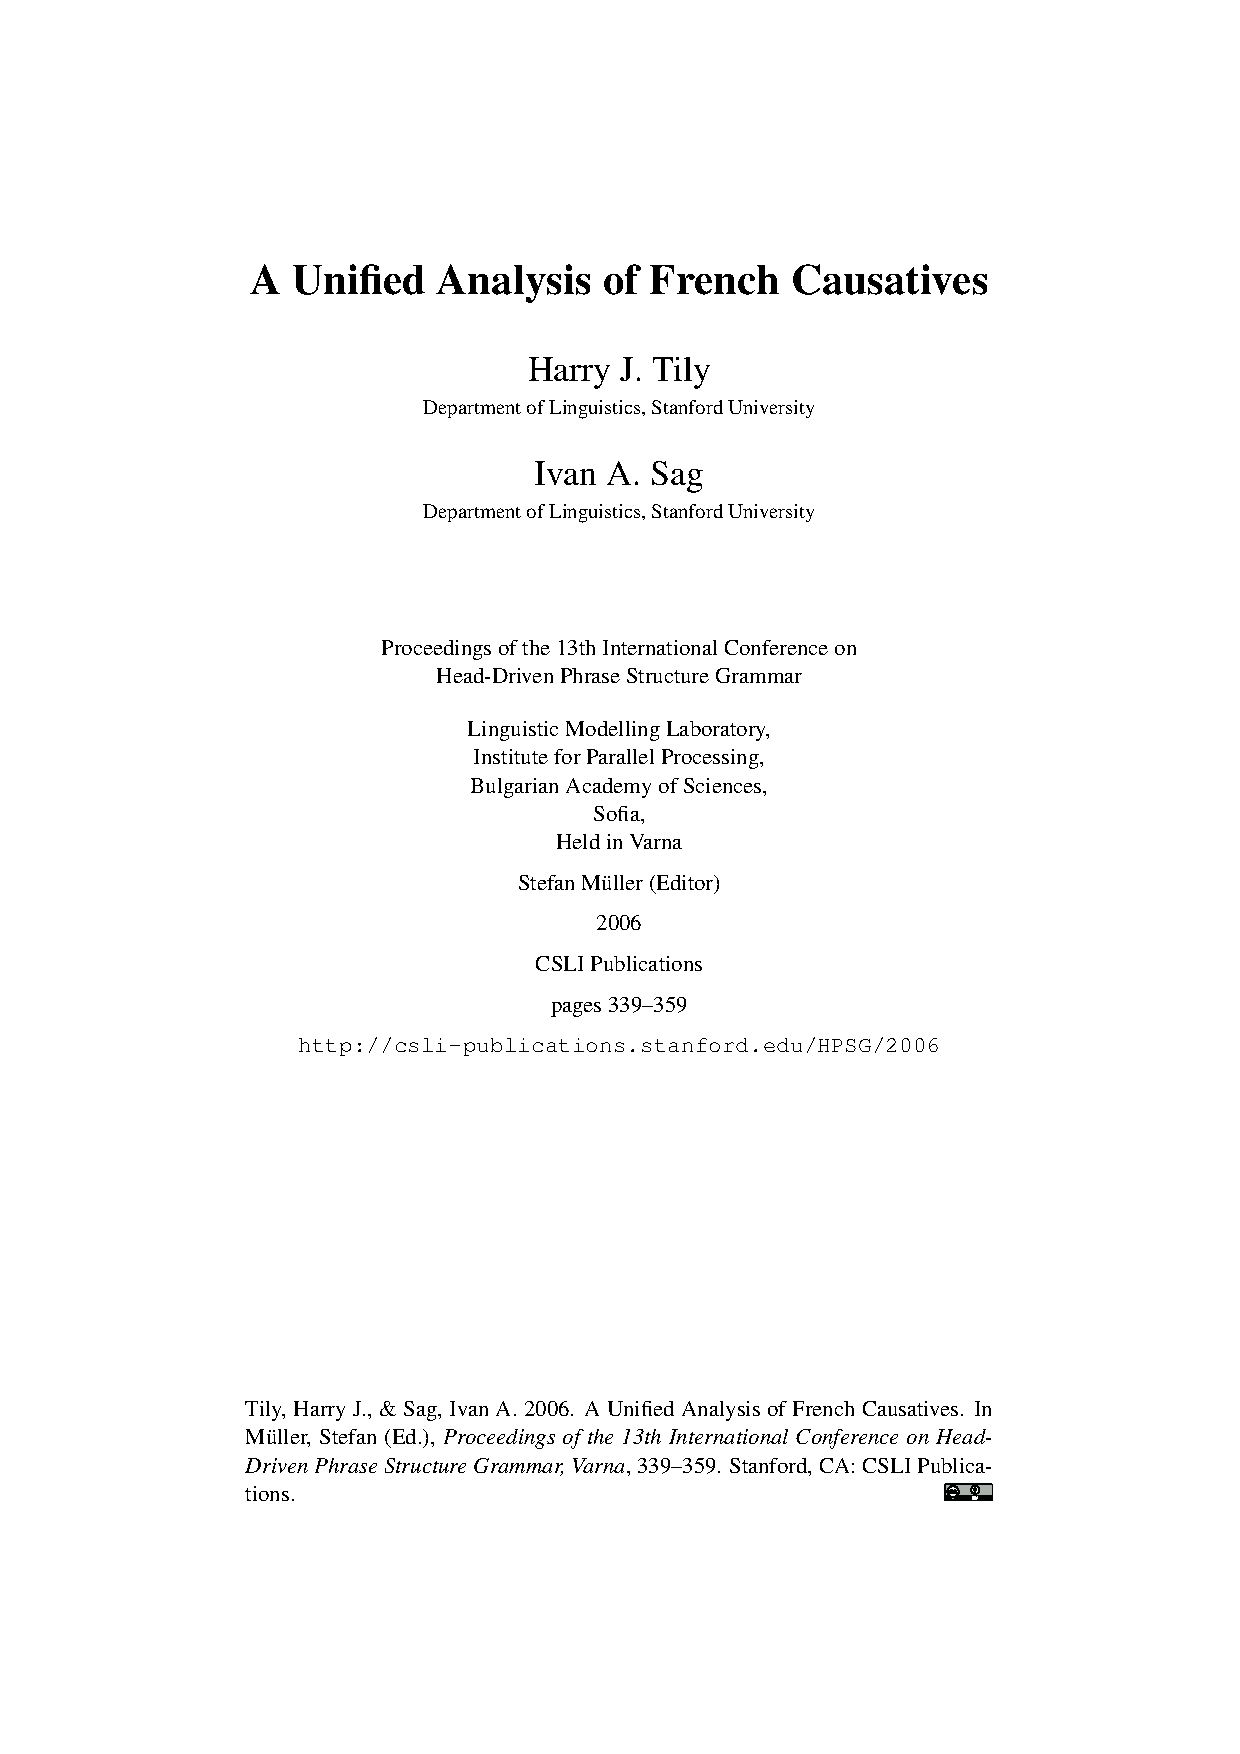
\includepdf[pages=-,pagecommand=\thispagestyle{plain},
            addtotoc={1,section,1,
            {Harry J.\ Tily and Ivan A.\ Sag: A Unified Analysis of French Causatives},
             ts}]{tily-sag.pdf}

\newpage
\part{Contributions to the Workshop on \emph{Regularity and Irregularity in Grammar and Language}}


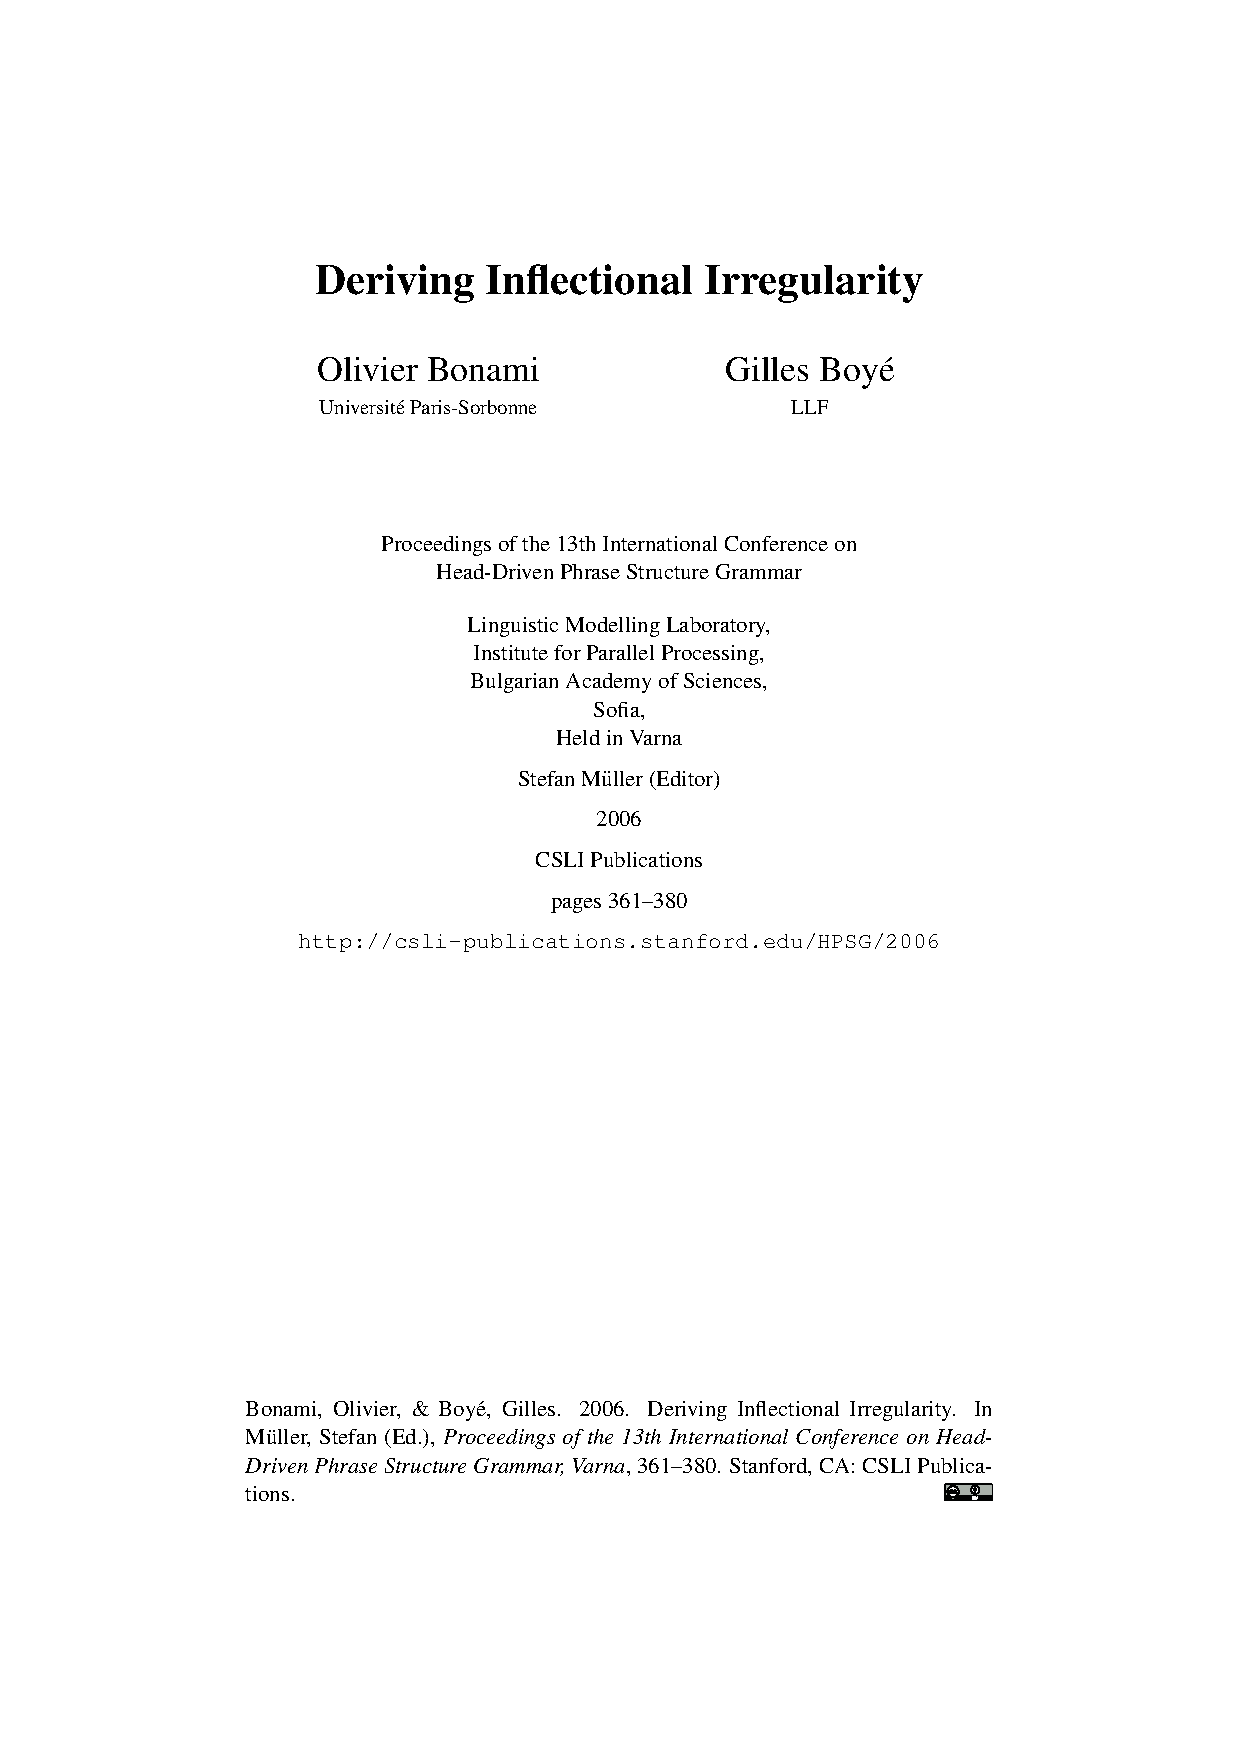
\includepdf[pages=-,pagecommand=\thispagestyle{plain},
            addtotoc={1,section,1,
            {Olivier Bonami and Gilles Boy�: Deriving Inflectional Irregularity},
             bonami-boye}]{bonami-boye.pdf}

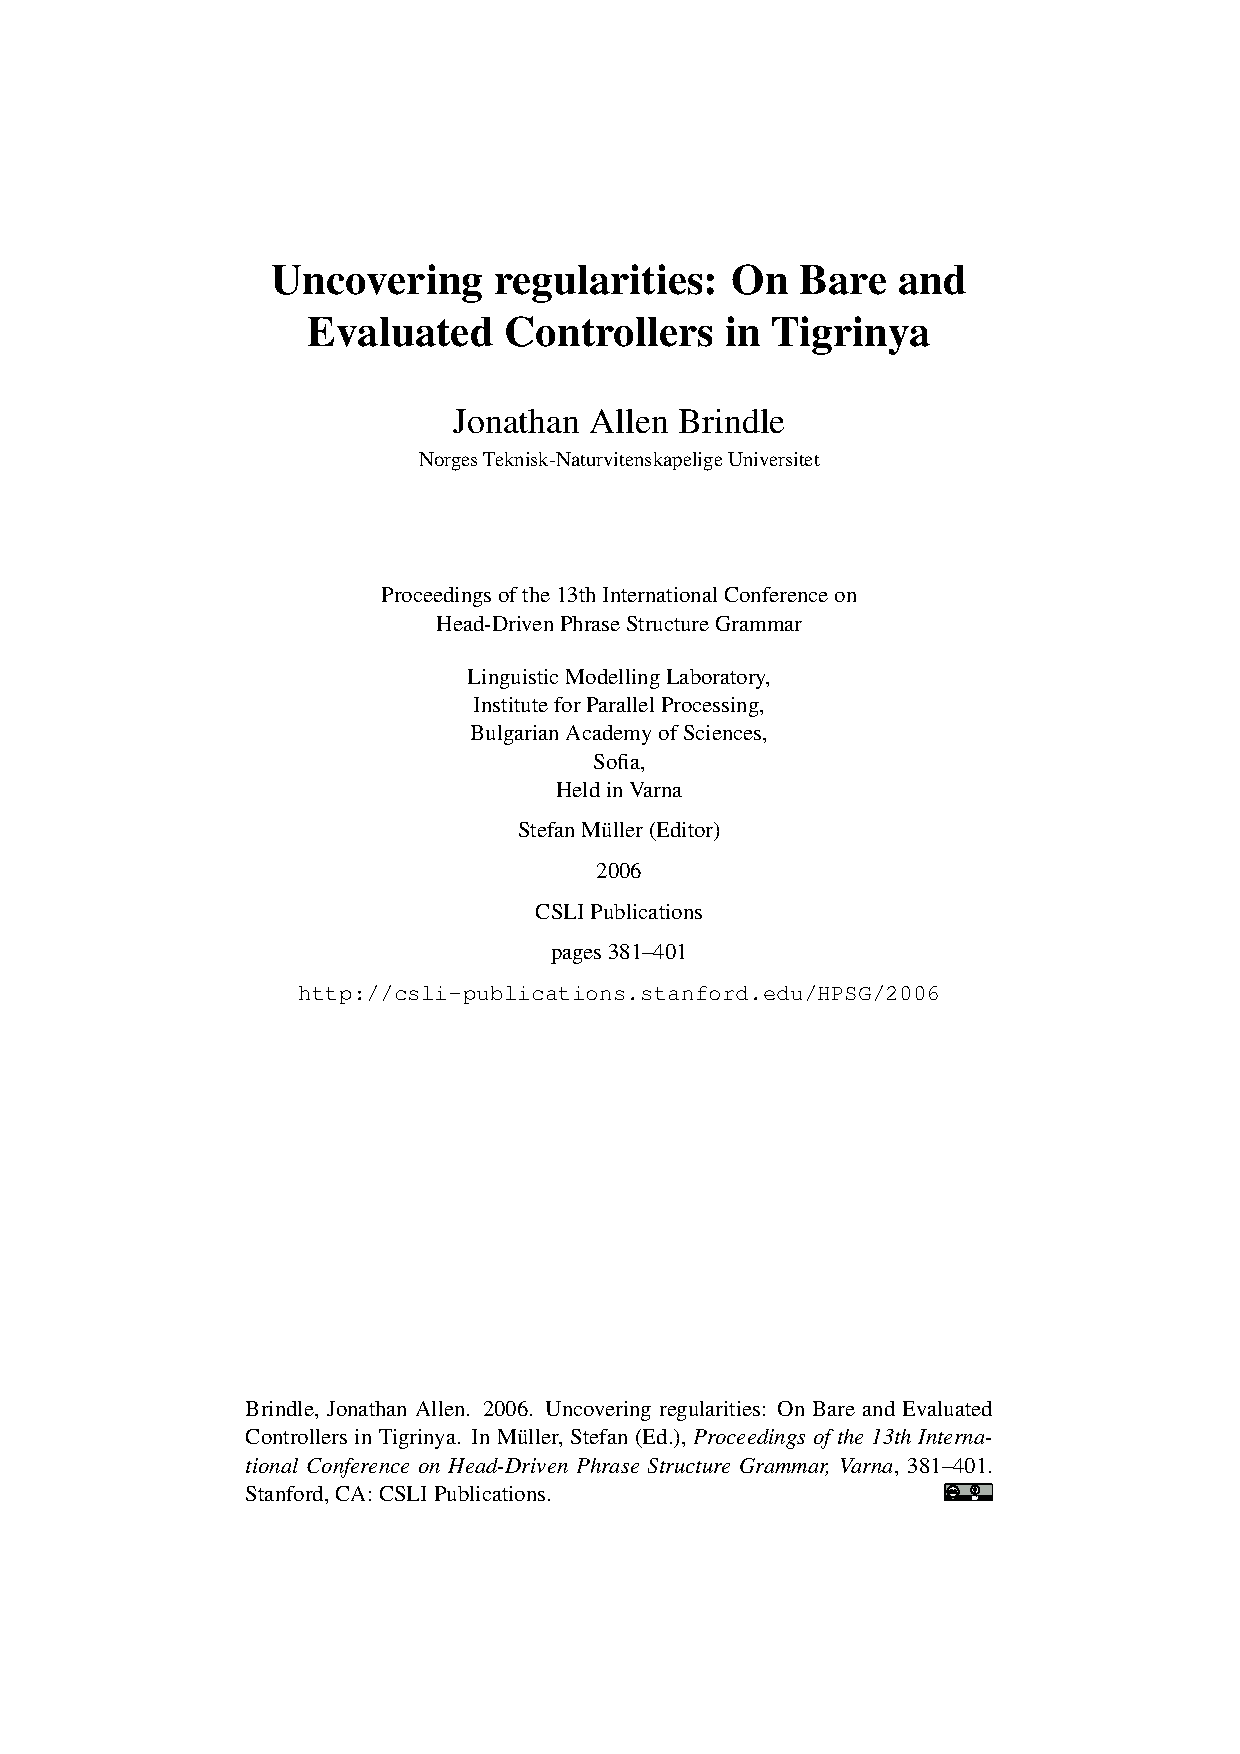
\includepdf[pages=-,pagecommand=\thispagestyle{plain},
            addtotoc={1,section,1,
            {Jonathan Allen Brindle: Uncovering regularities: On Bare and Evaluated Controllers in Tigrinya},
             brindle}]{brindle.pdf}

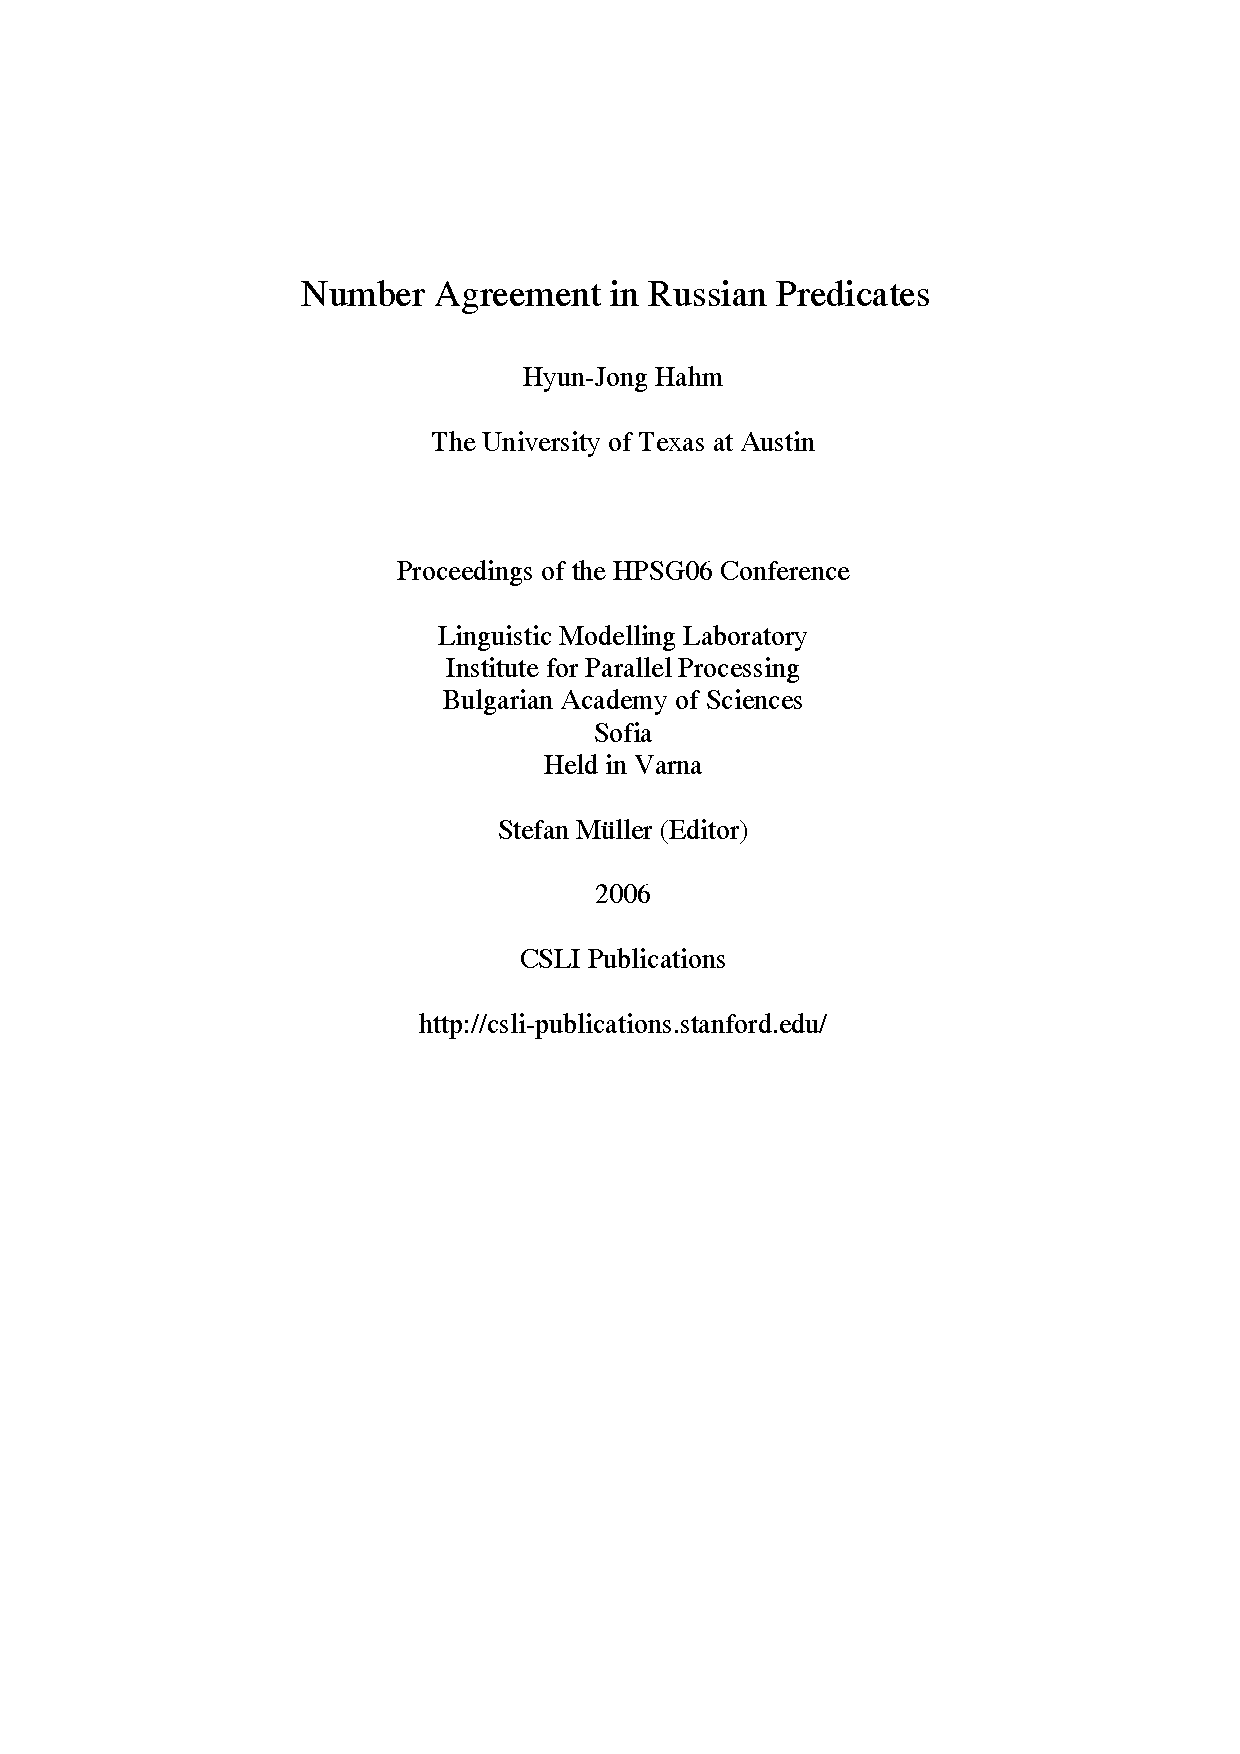
\includepdf[pages=-,pagecommand=\thispagestyle{plain},
            addtotoc={1,section,1,
            {Hyun-Jong Hahm: Number Agreement in Russian Predicates},
             hahm-r}]{hahm-russian.pdf}

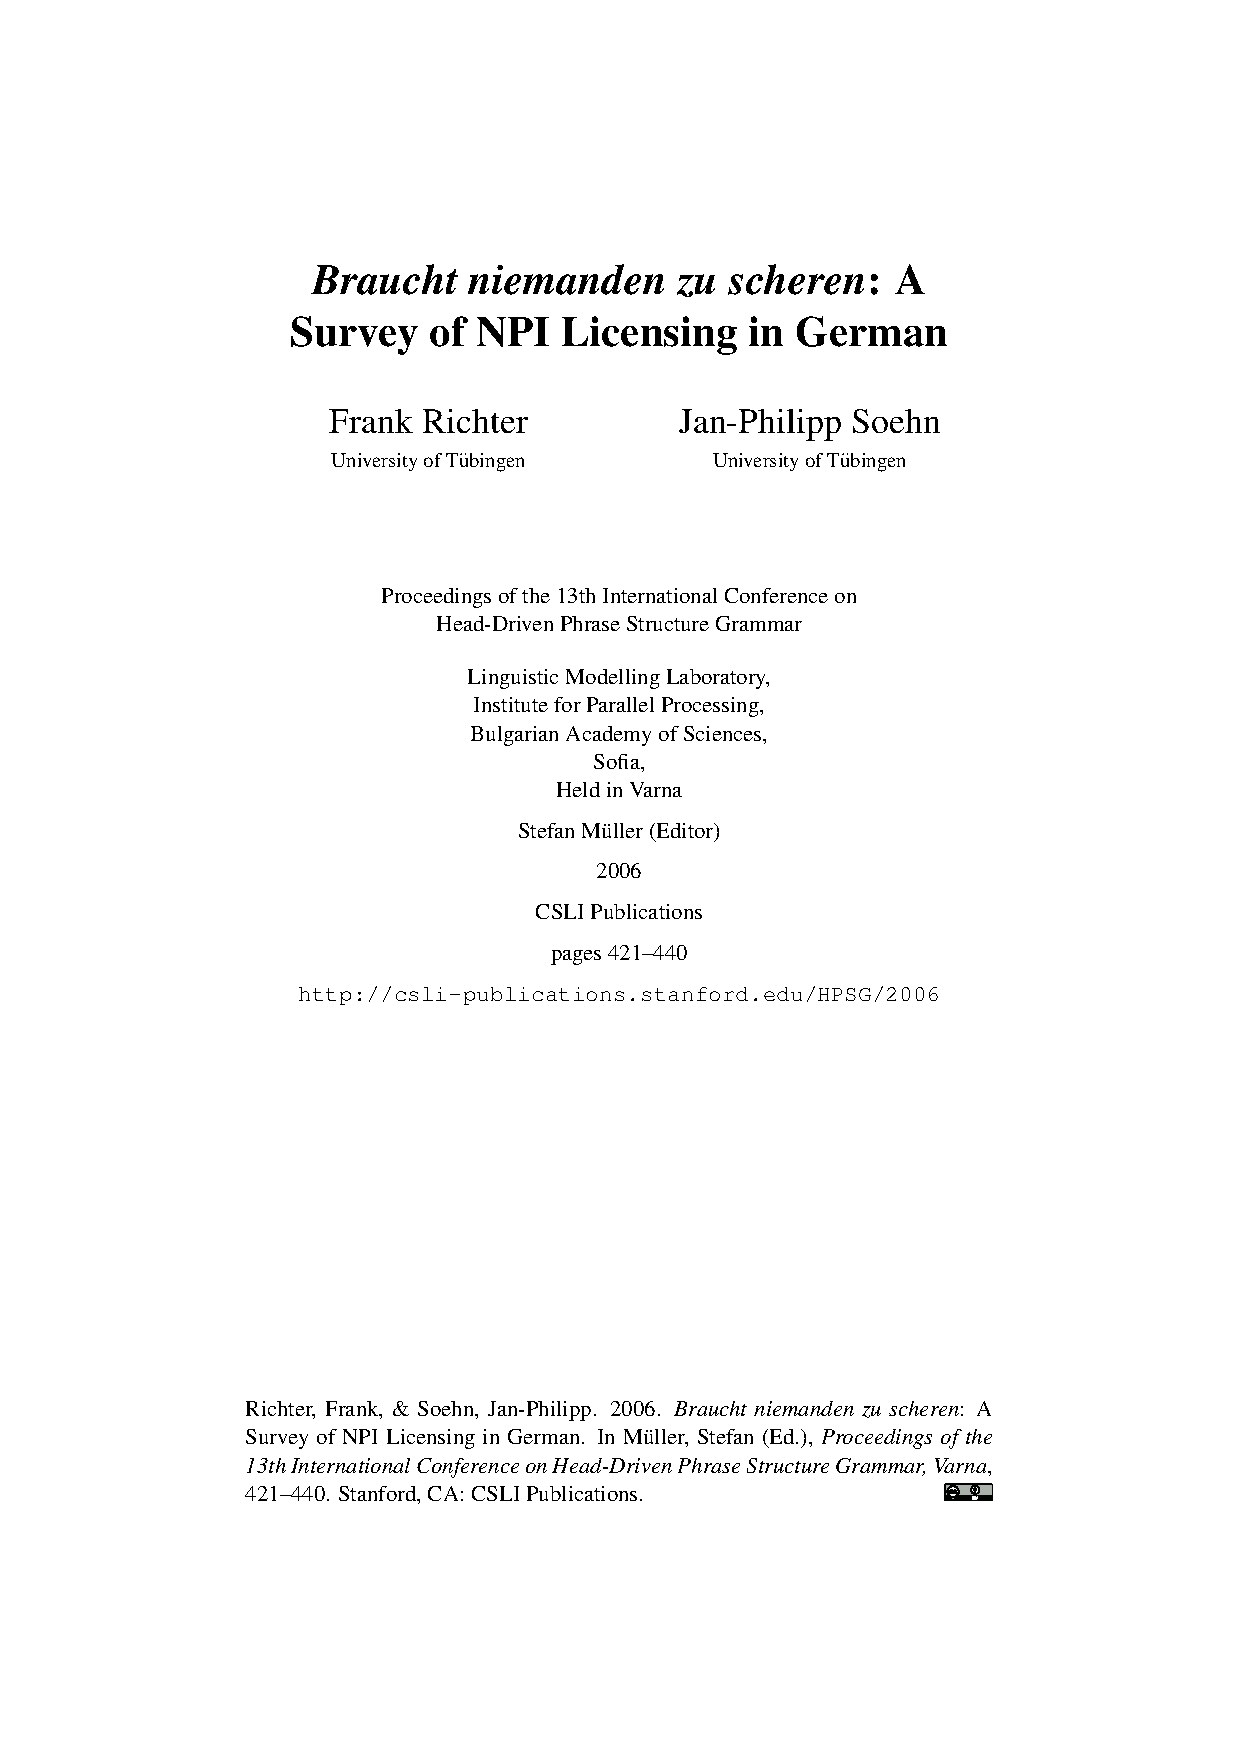
\includepdf[pages=-,pagecommand=\thispagestyle{plain},
            addtotoc={1,section,1,
            {Frank Richter and Jan-Philipp Soehn: \emph{Braucht niemanden zu scheren}: A Survey of NPI Licensing in German},
             rso}]{richter-soehn.pdf}

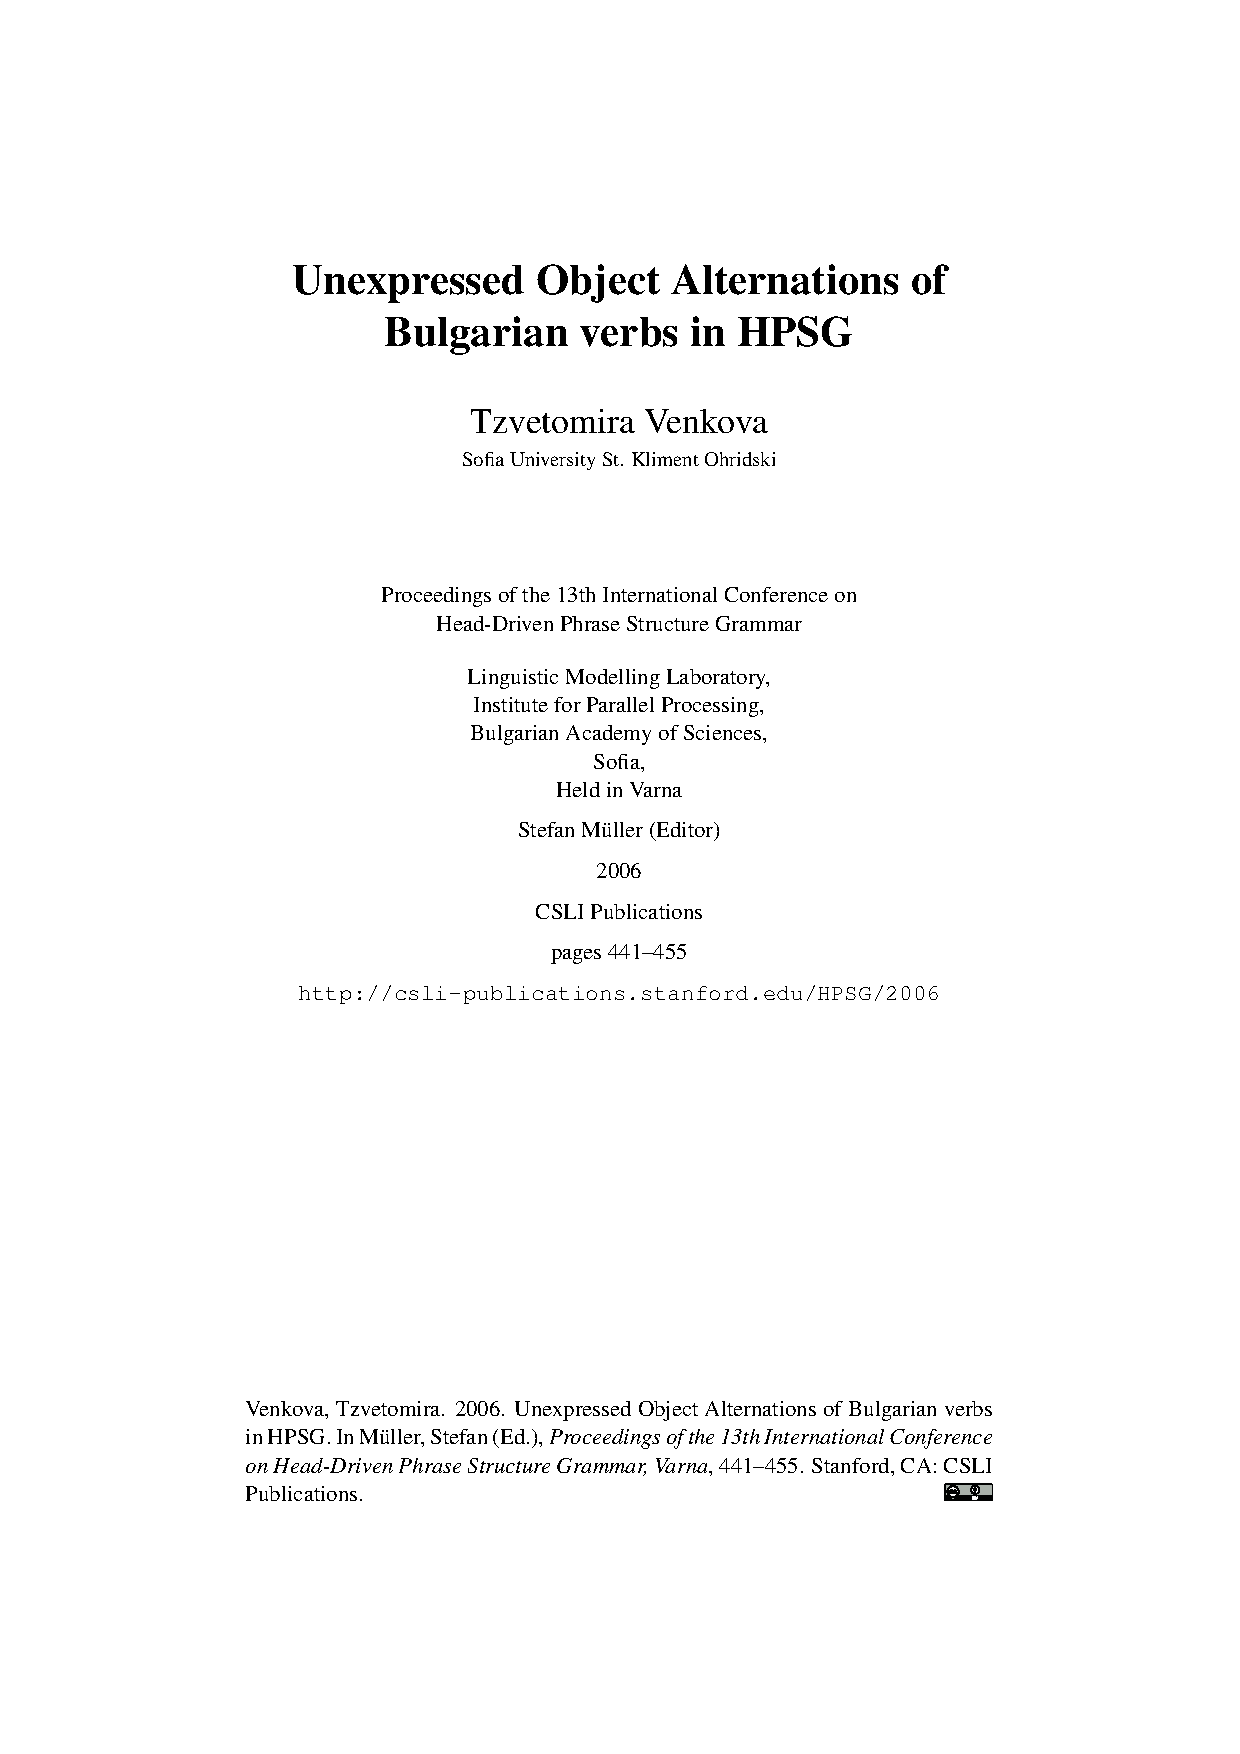
\includepdf[pages=-,pagecommand=\thispagestyle{plain},
            addtotoc={1,section,1,
            {Tzvetomira Venkova: Unexpressed Object Alternations of Bulgarian verbs in HPSG},
             venkova}]{venkova.pdf}




\end{document}

